\documentclass{article}
%\usepackage[utf8]{inputenc}
\usepackage{geometry}
\usepackage[utf8]{inputenc}    % allow utf-8 input
\usepackage[T1]{fontenc}       % use 8-bit T1 fonts
\usepackage{hyperref}          % hyperlinks
\usepackage{url}               % simple URL typesetting
\usepackage{booktabs}          % professional-quality tables
\usepackage{amsfonts}          % blackboard math symbols
\usepackage{amsmath}
\usepackage{nicefrac}          % compact symbols for 1/2, etc.
\usepackage{microtype}         % microtypography
\usepackage[pdftex]{graphicx}  % Use package of graphicx
\usepackage{tabularx}
\usepackage{comment}
\usepackage{amssymb}
\graphicspath{{figures/}}
\usepackage[english]{babel}
%\usepackage[table]{xcolor}
\usepackage{subfig}
\usepackage[ruled,vlined]{algorithm2e}
\usepackage{algorithm}
\usepackage{algorithmic}
%\usepackage{subcaption}
\usepackage{fullpage}

\graphicspath{{Images/}}
\title{Learning Hyperspectral Image Collections for Robust Classification}
\author{Chandrajit Bajaj, Akshay Varanasi, Tianming Wang}
\date{}

\begin{document}
\maketitle

\tableofcontents
\newpage

\section{Steps for Multi-target Identification/Multi-label Classification}
\begin{enumerate}
    \item Targets are categories Ex $T_1, T_2..$ where $T_1$ = animals and $T_2$=vehicles.For each $T_i \in [0,1] $ such that $0-t_1 \implies \text{class 1}, t_1-t_2 \implies \text{class 2}, .. $  where classes can be dog($class 1$),cat($class 2$) within animal category($T_1$). So this can be thought of as matrix $T_{i,j}= i^{th} \text{category},j^{th}\text{label/class}$. All categories may not have same number of classes or labels so we deal with this by having same number of columns or number of elements in row  for all categories. We bin the elements in each row vector according to number of classes in each category. This is Prior, so we have it.  
    \item Learn the Multi-level sparsity and spatial-spectral signature of all object classes for each target category in each image. This involves learning the statistics of the targets appearing in each image. \textbf{Training phase}
    \item Construct a reduced template or signature that allows for discriminating inter-target and intra-target. Learn the dictionary for discrimination in optimal space. Learn the Kernel for classification.\textbf{Training phase} 
    \item Develop Multi-level sampling of the Image occuring in the learned distribution of collection in 2.
    \item For each sample we test for recoverability of function(approx) 
    in a finite number of support region (can be boxes or ellipse) around sample point. So as to detect occurrence of target having class. 
    \item Refine if necessary the samples in the support region for $\epsilon$- function approximation.
    \item Classification or Identification of the target object using learned dictionary and kernel.
\end{enumerate}

\section{Things to keep in mind for Sampling}
\begin{enumerate}
    \item \textbf{Understanding the Signal and noise distribution/model in the images:} To learn sampling on the training data to get images so that they are representative. Learn the noise model as well along with signal model so that we can find co-variance of noise and consider it while sampling \\
    
    \textbf{Problem statement} 1. Which method or what do we measure or how to know the distribution? Example: We can use expectation maximization to know the distribution. 
    2. We need to know the parameters such as mean, variance etc from the distribution. 
    
    Assuming a dataset of grayscale images with width w and height h, each image is a sample outcome and a multivariate random variable is defined such that it assigns a w*h dimensional vector to each image where elements correspond to pixel values in the image. Suppose we have k classes then we can write the distribution as
    
    \begin{equation}
        p(\theta|v) = \sum^{k}_{i=1} \phi_{i}\mathcal{N}(\mu_{i},\Sigma_{i})
    \end{equation}
                                                                                                                                                                                                                                                                                                                                                                                                                                                                                                                                                                                                                                                                                                                                                                                                                                                                                                                                                                                                                                                                                                                                                                                                                                                                       
    where $\mu_{i}$ is a vector of length w*h. If $v \in \mathcal{N}(\mu_{i},\Sigma_{i})$ then 
    
    \begin{equation}
        p(v,\mu,\Sigma) = \frac{1}{\sqrt{(2\pi)^{n}\Sigma}}exp(-\frac{1}{2}(v-\mu)^T\Sigma^{-1}(v-\mu)) 
    \end{equation}
    
     We can use EM algorithm to find the parameters. We sample from this such that we get good training subset. We must include more images which are difficult to detect 
    
    \item \textbf{Learn to do Multi-level sampling:} We learn to do Multi-level sampling from training data of the desired domain such that we get a good approximate recovery. So when we solve the following recovery problem
    
    \begin{equation}
        \min ||X||_{*} \quad \text{ s.t } \quad P_{\Omega}(X) = P_{\Omega}(M) \quad \quad \text{ Matrix Recovery Problem}
    \end{equation}
    
    We get $X_{min}$ such that $||M-X_{min}|| \leq C||M||$ where $P_{\Omega}()$ is   the sampling which we designed. We want to do this in Multi-level fashion so $y = P_{\Omega} \Psi f$ then f can be recovered with recovery problem 
    
    \begin{equation*}
        \min_{z \in \mathbb{C}^N} ||z||_{1} \quad \text{subject to} \quad ||y - P_{\Omega} U z|| \leq \eta
    \end{equation*}
    
    where $\eta$ is chosen according to the noise level, $U = \Psi \Phi^*$. 
    
    \textbf{Problem statement:} 1. To know about Multi-level sampling parameters like how many levels, which basis to chose.
    2. And how many samples to sample given the error bound such that remaining samples can be sampled using leverage scores. Need to figure out how to do two-phase sampling
    

    \item \textbf{Low rank decomposition:} We want to get a low rank decomposition such that $CUR$
    
    \begin{equation}
        ||A-CUR||_{F} \leq ||A-A_{k}||_{F} + \epsilon ||A||_{F}
    \end{equation}
    
    \textbf{Problem statement:} We need to know which algorithm is best in terms of speed and accuracy. What are its error bounds. And instead of sampling based on leverages score calculated on the whole data, it should be calculated on random samples.
    
\end{enumerate}

\section{Choosing dataset}

Look at all the datasets and put their images

\subsection{HSI}
Hyperspectral datasets which we have are Indian pines,University of Pavia, Salinas dataset.

\subsection{Kimia}

This dataset contains digital pathological scan images.  
\section{Noise estimation}

\section{Statistics of HSI}

Explored various representations of “real-world” HSI. Example images are shown below. The entire image was divided into patches and properties of each patch was considered independently.

Let X[n,l] be an random P×P×B HSI patch, where n∈[1,..P]2 and l∈[1,..B]. 
We wish to express it in terms of orthonormal basis set Vi[n,l] and scalar co-efficients xi.
X[n,l] = μ[n,l]+∑xiVi[n,l]
PCA was used to learn the basis vectors.
Top 20 components rendered in RGB, as well as the plot of variance of for 200 components  is shown in the image.
Top 20 basis vectors account for 99% of variance

Since the basis set obtained had similar spatial patterns different spectra or colors, separable basis was also explored. The basis was decomposed into a Cartesian product of separate spatial and spectral components.
Vi[n,l]=Sj[n]Ck[l] where Sj[n] and Ck[l] are orthonormal bases.
First few spatial and spectral components are shown in the figure.


Learned separable basis is compared to general PCA basis in terms of reconstruction error.  

Where X0:i is the estimate of X reconstructed using only the first i components.
A wavelet-based separable basis, with the spatial components Sj corresponding to Haar wavelets, is also included for comparison and the result is shown in the next slide. 

We see that error curves of general and separable basis match almost exactly.

Variance along their separable components is looked and it is found out that the total variance in the different spatial components is distributed in similar proportions along the spectral dimension.

Top 15 general PCA basis is expressed in terms of separable basis as shown in the table.
This gives us another way of looking at variance ( since it is related to general pca basis)
It was found that that combinations of the first spectral component with various spatial components have higher variance than the latter spectral components. 

After identifying the separable basis, distribution of coefficients  was looked upon. 
Let xjk be the coefficient of X in the basis component Sj[n]Ck[l]
Looking at the empirical distribution of x1k , we see that they lack structure.
In applications with grayscale and RGB images, (“scaling”) coefficients are found to be poorly described by standard probability distributions and are often simply modeled as being uniform and the same could be done here.     

The statistics of the higher spatial coefficients(xjk for j > 1) are more interesting as we can see in the figure, the distribution of  x21  and x22 
 We see that these distributions are zero-mean,uni-modal, symmetric, and more kurtotic than a Gaussian distribution with the same variance, with heavier tails and a higher probability mass near zero.
Gaussian mixture model was used to model as they allow tractable inference. 

We define such model as

where zjk ∈ {1,... Z} is a latent index variable indicating that xjk is distributed as a Gaussian with the corresponding variance σ2jk,z.
The model parameters {p(zjk = z);  σ2jk,z  }z are estimated from the database using Expectation Maximization (EM)  and in practice we find that a mixture of 8 Gaussians (i.e., Z = 8) provides accurate fits to the empirical distributions for all coefficients.

Since the spatio-spectral basis vectors have been estimated through PCA, it follows that xjk and xjk’ will be uncorrelated for k ≠ k’, i.e. E(xjkxjk’) = 0.
Different spatial coefficients at the same spatial location in grayscale images are known to be related. Similarly different spectral coefficients along the same spatial basis are also mutually dependent, and a model that encodes these dependencies is proposed.

So whether knowing the value of the mixture index zjk carries any information about the statistics of the coefficient xjk’ for a different spectral component k’ along the same spatial basis j is what is to be explored.






















\section{Statistics of natural image categories}

In this paper we study the statistical properties of natural images belonging to different categories and their relevance for scene and object categorization tasks. We discuss how second-order statistics are correlated with image categories, scene scale and objects. We propose how scene categorization could be computed in a feedforward manner in order to provide top-down and contextual information very early in the visual processing chain. Results show how visual categorization based directly on low-level features, without grouping or segmentation stages, can benefit object localization and identification. We show how simple image statistics can be used to predict the presence and absence of objects in the scene before exploring the image.

According to the seminal work of Rosch and collaborators (1976), people recognize most of the objects at the same level of abstraction: the basic level (e.g. car, chair). It has been shown that objects of the same basic-level category share similar common features and usually they have a similar shape.  In each prototype image, information about the level of spatial similarity existing between local features (e.g. distribution of coloured regions and intensity pattern) is demonstrated by the degree of sharpness. Similarly to objects, natural images depicting environmental scenes can also be classified
in basic-level categories (Tversky and Hemenway 1983), and as such, are expected to share common features (Jepson et al 1996).  A strong relationship exists between the category of a scene picture and the distribution of coloured regions in the image. In a similar vein, the distribution of structural and colour patterns of the background scene around an object is constrained.  

Because of the correlation existing between an object and its context the background does not average to a uniform field (Torralba 2003). On the contrary, the background exhibits the texture and colour pattern that is common to all environments where a specific object is usually found  Because different environmental categories are built with different objects and materials,and the point of view of the observer imposes its own constraints (such as its size and motion), we expect to find strong biases in the statistics distribution of the image information. Those statistics might have different biases for different animal species. In this paper, we illustrate how simple statistics of natural images vary as a function of the
interaction between the observer and the world.

spectral principal components of natural images and scene-tuned
filters, and describe how these methods could be used to perform simple scene categorization
tasks. 

computational approaches of scene categorization, and section 6
shows the robustness of simple statistics in performing object detection tasks.

\textbf{Spectral signatures of image categories}
Different categories of environments also exhibit different orientations and spatial frequency distributions, captured in the averaged power spectra (Baddeley 1997, Oliva et al 1999, Oliva and Torralba 2001). Figure 3 shows that the differentiation among various man-made categories resides mainly in the relationship between horizontal and vertical contours at different scales, while the spectral signatures of natural environments have a broader variation in spectral shapes.

\subsection{Principal components of real-world images and power spectra}

Principal component analysis (PCA) has been extensively used in vision problems for coding and recognition. In the face recognition domain, when faces are correctly aligned and scaled, PCA gives a reduced set of orthogonal functions able to reconstruct faces.(Craw and Cameron 1991, Turk and Pentland 1991). Image principal components (IPCs) decompose the image as 
\begin{equation}
    i(x,y) = \sum^{P}_{n=1}v_{n}IPC_n(x,y)
\end{equation}

where i(x, y) is the intensity distribution of the image along spatial variables x and y. $P \leq N^2$
is the number of total IPCs and $N^2 = 256^2$ is the number of pixels of the image. The $IPC_n(x, y)$ are the eigenvectors of the covariance matrix: $T = E[(i-m)(i-m)^T]$, where i are the pixels
of the image rearranged in a column vector. E is the expectation operator. $m = E[i]$ is the mean of the images. $v_n$ are the coefficients for describing the image i(x, y). As discussed by Field (1994),
stationarity of natural images is responsible for IPC shape (figure 8(a)) which corresponds to the Fourier basis.

Here, we compute the power spectrum of an image by taking the squared magnitude of its discrete Fourier transform (DFT):

\begin{equation}
    \Gamma(k_x,k_y) = \frac{1}{N^2}|I(k_x,k_y)|^2
\end{equation}
where
\begin{equation}
    I(k_x,k_y) = \frac{1}{N^2}\sum^{N-1}_{x=0}\sum^{N-1}_{y=0}i(x,y)exp(-\frac{j2\pi}{N}(xk_x+yk_y))
\end{equation}

$f_x = k_x/N$ and $f_y = k_y/N$ are the discrete spatial frequencies. The power spectrum4,$\Gamma(k_x, k_y)$, encodes the energy density for each spatial frequencies and orientations over the
whole image. PCA applied to power spectra gives the main components that take into account the structural variability between images. First, the power spectrum is normalized with respect
to its variance for each spatial frequency: $(k_x, k_y) = \Gamma(k_x, k_y)/std[\Gamma(k_x, k_y)]$, with
$std[\Gamma(k_x, k_y)] = \sqrt{E[(\Gamma(k_x, k_y) - E[\Gamma(kx, ky)])^2]}$. This normalization compensates for the
$1/f^{\alpha}$ shape of the power spectrum. The spectral principal components (SPCs) decompose the
normalized power spectrum of an image as
\begin{equation}
    \Gamma_s'(k_x,k_y) = \sum^P_{n=1}u_n SPC_n(k_x,k_y)
\end{equation}
P is the number of SPCs.

The three first principal components exhibit vertical and horizontal spectral component dominance. 

 An organization of broad environmental categories emerges, suggesting that the variability in the second-order statistics of natural images may be relevant for natural scenes classification tasks.A linear combination of the first three SPCs is able to separate man-made scenes from natural
scenes with an accuracy of 80\%.

\subsection{Receptive fields for scene recognition}

In this section, we look for the best spectral statistics providing discrimination between man-made, natural, open and closed scene categories. Linear discrimination between two scene categories, using the normalized image power spectra $\Gamma(k_x, k_y)$, can be achieved as

\begin{equation}
   w = \sum^{N-1}_{k_x=0} \sum^{N-1}_{k_y=0} \Gamma'(k_x,k_y)DST(k_x,k_y) =  \sum^{N-1}_{k_x=0} \sum^{N-1}_{k_y=0} \Gamma(k_x,k_y)DST'(k_x,k_y)
\end{equation}

with $DST'(k_x,k_y)= DST(k_x,k_y)/std[\Gamma(k_x,k_y)]$

$DST'(k_x,k_y)$ is the weighing of the spectral components needed to discriminate between the two classes (DST standing for discriminant spectral template). w is the most discriminant feature and is obtained as a weighted sum of the power spectrum of the image. As SPCs define
a complete orthogonal basis for describing the normalized power spectra, we can write the DST as
\begin{equation}
    DST(k_x,k_y) \approx \sum^P_{n=1} a_n SPC_n(k_x,k_y)
\end{equation}

The coefficients $a_n$ indicate how to weight of each SPC in order to build a specific template
DST. Here, we used the first P = 16 SPCs. The coefficients an are determined by a supervised
learning stage. In the learning stage, each image is represented by a column vector of features
$u = {u_n}, u_n$ being the projection of the power spectrum of the image into the nth SPC.  The parameters of the DST, an, can be learnt by applying Fisher linear discriminant analysis (e.g. Ripley 1996,
Swets and Weng 1996) that looks for the coefficients $a_n$ giving the best classification rate.

Due to the linearity of equation (6), the discrimination performed in the
spectral domain (DST') can be written in the spatial domain. It is then possible to compute
receptive fields tuned to global scene statistics that discriminate between the categories of
natural scenes.
The output energy of a discrete filter with transfer function $H(k_x, k_y)$ can be computed as

\begin{equation}
   E = \sum^{N-1}_{k_x=0} \sum^{N-1}_{k_y=0} \Gamma(k_x,k_y)|H(k_x,k_y)|^2
\end{equation}

This expression is similar to equation (6) used to compute the structural feature w. However, as the squared magnitude of the transfer function of a filter cannot have negative values, the DST' can be implemented by computing the difference between the output energies of two filters.
In such a case, we can compute w as the difference between two energies as $w = E_{+}- E_{-}$ where $E_{+}$ and $ E_{-}$  are respectively the output energy of two filters with transfer functions  $H_{+}$ and $ H_{-}$. In such a case, we obtain

\begin{equation}
   w = \sum^{N-1}_{k_x=0} \sum^{N-1}_{k_y=0} \Gamma(k_x,k_y)(|H_{+}(k_x,k_y)|^2-|H_{-}(k_x,k_y)|^2)
\end{equation}

With this expression, it is possible to obtain positive and negative values for DST'. Several functions $H_{+}$ and $ H_{-}$ give the same resulting DST'. Here, we use
\begin{equation}
    |H_{+}(k_x,k_y)|^2 = rect[DST'(k_x,k_y)]
\end{equation}

and

\begin{equation}
    |H_{-}(k_x,k_y)|^2 = rect[-DST'(k_x,k_y)]
\end{equation}

where rect(x) is a half rectifying function: rect(x) = x if x > 0 and rect(x) = 0 if x < 0.
These equations give the magnitude of the two filters. As the phase can be freely chosen, we chose null phase filters as this allows us to obtain filters with spatial localized impulse response. The impulse responses of these two filters are receptive fields that best discriminate between two groups of images.

If we compute the output of the two filters by convolution of the image with the respective impulse responses, $o_{+}(x,y)=i(x,y)*h_{+}(x,y) $ and $o_{-}(x,y)=i(x,y)*h_{-}(x,y)$, then the structural feature can be also obtained as

\begin{equation}
   w = \sum^{N-1}_{k_x=0} \sum^{N-1}_{k_y=0} \Gamma(k_x,k_y)(|o_{+}(x,y)|^2-|o_{-}(x,y)|^2)
\end{equation}

We define an opponent energy channel as the image obtained by the difference $d(x, y) = |o_{+}(x, y)|^2 - |o_{-}(x, y)|^2$. This signal gives the spatial locations that contribute to the
discriminant feature w.

\subsection{Semantic categorization}
scene recognition as a process that combines a set of image-based features (e.g. colour,orientation, texture) to form higher-level representations such as regions (blobword from Carson et al 2002), simple blocks (geons from Biederman 1987) or objects (Barnard and Forsyth 2001)

The consequence of a system that would compute ‘high-level scene’ primitives directly from a basis of low-level features is appealing to theoretical and computational issues of recognition. If robust scene categorization could be computed in such a feedforward manner (Van Rullen and Thorpe 2001), it would provide top-down and contextual information very early in the visual processing chain that could prove beneficial to object localization, segmentation and identification processes. 

\subsection{Image Statistics and contextual object processing} 

As suggested in the introduction, the global image statistics are also correlated with the objects present in the scene. This is not just because the object shape has an impact on the global image statistics (when the object is small this effect is negligible), but also because there exists
strong correlation between the objects present and their context.

 The average pictures show the mean intensity values and the spectral signature of the scene pictures that contain each object. Although no other constraints are imposed, the different average pictures correspond
to the signatures of the environments that are the typical context of the objects selected. For instance, animals are expected to be in natural environments. Cars are found in roads and urban environments.  

these scenes are characterized by particular global image statistics.
Using image statistics provides a way of introducing contextual information in object detection approaches that does not require the detection of other objects. For the prediction of
the presence/absence of an object of interest we use a statistical framework more reliable than the linear discrimination performed in section 4. The function $P(O| v_C)$ gives the probability
of presence of the object class O given a set of global image statistics $v_C$ that represent the
contextual information.
The training set used for learning the probability $P(O|v_C)$ is a set of annotated pictures. We use Bayes rule to write $P(O|v_C)  = P(v_C|O)P(O) + P(v_C|\hat{O})P(\hat{O})$. We learn the PDF $P(v_C|O)$ from a set of images in which the object is present. We approximate the PDF using
mixtures of Gaussians and the learning is performed using the EM algorithm (Torralba and Sinha 2001). In the same way, we learn the PDF $P(v_C|O)$ using a set of images in which
the object is absent. We assume that $P(O) = P(\hat{O}) = 1/2$. The contextual features $v_C$ are the features obtained by projecting the image power spectra into the first 16 SPCs. Once the learning is done, the function $P(O|v_C)$ evaluates the consistency of the object O with the context $v_C$ and, therefore, provides information about the probable presence/absence of one object category before scanning the picture looking for the object.

Image statistics can also predict other object properties such as scale (due to the correlation between scene scale and image statistics) or its location in the scene. For instance, we can learn the statistical relationship between the location of faces in an image (x) and the global
image statistics $(v_C):P(x|v_C)$. In order to be able to have access to spatial information we include in the image features $v_C$ the spectral features computed at several locations in the age. Specifically, we divide the image in 4 $\times$ 4 patches and we compute the power spectra at each patch. This allows us also to encode in $v_C$ information about the spatial organization of the image (Oliva and Torralba 2001).
The learning of the probability density function $P(x|v_C)$ provides the relationship between the context and the more typical locations of the object of interest in the image. For modelling
this PDF we use a mixture of Gaussians (Gershnfeld 1999):
\begin{equation}
    P(x|v_C) = \sum^M_{i=1}b_i G(x;x_i,X_i)G(v_C;v_i,V_i)
\end{equation}


We learn the parameters of this model using the EM algorithm and a training database of annotated images (Torralba and Sinha 2001, Torralba 2002). This PDF formalizes one aspect of the contextual control of the focus of attention. When looking for faces (or any other object
of interest), attention will be directed into the candidate regions with the highest likelihood $P(x|v_C)$ of containing the target object, based on the past experience of the system. Note that although the contextual features encode the image using 4 $\times$ 4 patches, the variable x is a
continuous variable. Given $v_C$ from an image, the PDF $P(x,v_C)$, as a function of location x, will be a mixture of Gaussian blobs (figure 15)

\section{Compressive Sensing}
The goal is to learn the optimal sampling scheme such that we can work on the sampled data instead of the whole data. We can do that by Compressed sensing which is a signal processing technique for efficiently acquiring and reconstructing a signal, by finding solutions to under determined linear systems. Compressed sensing (CS), introduced by Candès, Romberg and Tao (1) and Donoho (2), states that under appropriate conditions one can overcome the Nyquist sampling barrier and recover signals
using far fewer samples than dictated by the classical Shannon theory. This has important implications in many practical applications
which caused CS to be intensely researched in the past decade.

Traditional CS is based on three pillars: sparsity (there are s important coefficients in the vector to be recovered, however, the location is arbitrary), incoherence (the values in the measurements matrix
should be uniformly spread out) and uniform random subsampling. All these are not valid in case where device imposes sampling operator leaving the freedom to chose sampling strategy to us, unlike the case where are both are free to chose.

There are different ways of acquiring/sampling and reconstructing a signal which will be discussed further in the following sections.

\section{CUR decomposition}

General assumption is that noise makes a the data full rank. In CUR decomposition, we try to get an low rank approximation of the matrix(A) expressed as product of three matices which reveal the structure. The classic,optimal approach is the singular value decomposition, $$A = U\Sigma V^{*}$$ with U and V having orthonormal columns, and $\Sigma$ diagonal. However, the orthonormal singular vectors aren't so representative of the data. Among suboptimal approaches called interpolatory factorizations, the best known example is the CUR decomposition.$$A = CUR$$, where C and R are taken from the columns and rows of A, so they are representative. The CUR can be computed using different strategies.

\begin{enumerate}
    \item Column pivoted QR factorizations 
    \item Volume optimization 
    \item Uniform sampling of columns 
    \item Leverage scores
    \item Empirical Interpolation approaches
\end{enumerate}

Among different algorithms for CUR decomposition, the following were used.

\subsection{Linear Time CUR}

First CUR algorithm named as LinearTimeCUR (LTCUR), is due to Drineas, Kannan and Mahoney[3]. This
method, presented in algorithm 1 , consists of three main steps: (1) first it constructs a matrix $C \in \mathbb{R}^{n \times c} $
by randomly sampling $c = O(k/ \epsilon^4)$ (or $c = O(1/ \epsilon^4)$ for spectral norm) columns of A in c independent identical
trials; in each trial column $A_{,j}$ is sampled with probability $p_j = ||A:,j||^2/||A||^2_ F$ and if it is picked, it is rescaled by $1/\sqrt{cp_j}$,  then it forms a matrix $R \in \mathbb{R}^{r \times d}$ by independently sampling $r = O(k/ \epsilon^2)$ rows of A proportional
to their squared norm; in each trial row $A_{i,:}$ is sampled with porbability $q_i = ||A_{i,:}||^2/||A||^2_F$, and if it is selected it is rescaled by $1/\sqrt{rq_j}$ and (3) finally it constructs matrix $U \in \mathbb{R}^{c \times r}$ as the intersection of C and R and properly rescales such that $A = CUR$.

They showed setting $c \geq 64k\mu^2_c/\epsilon^4$ and $r \geq 4k/\delta_r^2 \epsilon^2$ where $ \mu_c = 1 + \sqrt{8log (1/\delta_c)}$ and $0 \leq \epsilon \delta_r \delta_c \leq 1$, LTCUR achieves Frobenius error bound
\begin{equation}
    ||A - CUR||_F \leq ||A - A_k||_F + \epsilon||A||_F
\end{equation}

and setting $c \geq 64\mu^2_c/\epsilon^4$ and $r \geq 4k/\delta^2_r\epsilon^2$ it obtains spectral error bound as with probability $1-(\delta_r + \delta_c)$

\begin{equation}
    ||A - CUR||_2 \leq ||A - A_k||_2 + \epsilon||A||_F
\end{equation}


\subsection{Space and Run Time Analysis}
In LTCUR, clearly sampling probabilities $p_i$ and $q_j$ can be computed in one pass, $O(nd)$ time (for reading
data) and using $O(c + r)$ space. A second pass is needed to compute matrices $C, R and \Psi$; this will take
$O(nd + dc + nr)$ time (since sampling is with replacement and each d column $(n rows)$ of A can be selected
for all c columns $(r rows)$ of C (R)), also it needs $O(nc + dr + cr)$ additional space to store these three
matrices. Having C in hand, one can compute $C^T C$ and get rank k of that in $O(nc^2 + c^2k)$ time and $O(c^2)$
space. Therefore the total run time of algorithm 1 would be $O(nd + dc + nr + nc^2)$, and the space usage
would be $O(nc + dr + cr)$.


\subsection{Leverage Score CUR}
In this section, we describe LeverageScoreCUR( LSCUR) algorithm[4] which constructs matrices C and R based on “column leverage scores” and “row leverage scores” of input matrix A.

Recall that if $A = USV^T$ is SVD decomposition of $A \in \mathbb{R}^{n \times d}$, then one can write $j$-th column of $A$ as linear combination of all left singular vectors (column of $U$) rescaled by corresponding singular values and entries
of $j$-th row of right singular vector matrix (i.e. $V$ ); in other words
\begin{equation*}
    A_{:,j} = USV^T_{j,:} = \sum^n_{i=1}S_{i,i}U_{:,i}V_{j,i}
\end{equation*}
If we truncate this summation to first $k < n$ left singular vectors and values, we can approximate $A_{:,j}$ as

\begin{equation*}
    A_{:,j} \approx \sum^k_{i=1}S_{i,i}U_{:,i}V_{j,i}
\end{equation*}

We define the leverage score of $j$-th column as $score(A_{:,j}) =  \sum^k_{i=1} V_{j,i}^2 $. Note that sum of leverage scores for
all column of A is exaclty k:

Therefore in order to define sampling probabilities we normalize leverage scores as $p_j = \sum^k_{i=1} V_{j,i}^2$ ; with the normalization $\{p_j\}^d _{j=1}$ form probability distribution over columns of $A$ as $p_j \geq 0$ and $\sum^d_{j=1} p_j = 1$. Using these sampling probabilities, authors of [4] proposed the ColumnSelect algorithm (depicted in algorithm )
that samples $c = O(k log k/\epsilon^2)$ columns, forms a matrix $C \in \mathbb{R}^{n \times c}$ and achieve error bound $A - \pi_C(A)||_F \leq (1 + \epsilon/2)||A - A_k||_F$ The LSCUR which is described in algorithm 5.2.2 uses ColumnSelect algorithm on both $A$ and $A^T$ to achieve relative error bound $||A - CUR||_F \leq (2 + \epsilon)||A - A_k||_F$.

\begin{figure}
    \centering
    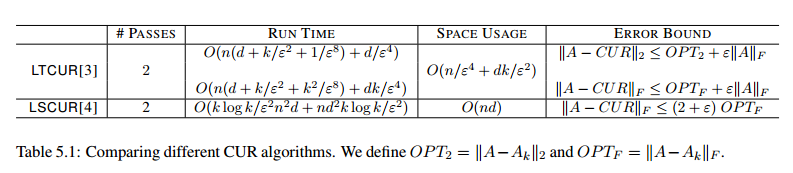
\includegraphics[width=0.75\textwidth]{Figures/cur_compare.png}
    \caption{Comparing different CUR algorithms}
    \label{fig:my_label}
\end{figure}
\subsection{Space and Run Time Analysis}

Since LSCUR needs to take SVD of input matrix, it loads the whole matrix into memory, which takes $O(nd)$
time to read data, and $O(nd)$ space to store it. Taking SVD of it costs $O(nd^2)$ additional time. In another pass over data, LSCUR constructs matrices $C$ and $R$, that takes $O(cd + rn)$ additional time and space. Finally
computing matrix $U$ requires $O(cn^2d + nd^2r)$ time and $O(cr)$ space. Overall LSCUR runs in $O(cn^2d + nd^2r)$
time and $O(nd)$ space


\begin{figure}[ht]
 \centering    
 \subfloat[Original image $(522 \times 775)$]{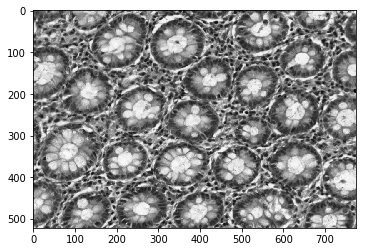
\includegraphics[width=0.45\textwidth]{Figures/original.png}\label{fig:sub1}}
 \end{figure}

\begin{figure}[ht]
 \centering    
 \subfloat[Using algorithm ]{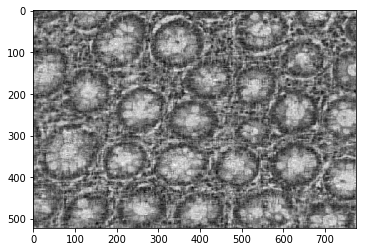
\includegraphics[width=0.45\textwidth]{Figures/CUR_100.png}\label{fig:sub2}}
\end{figure}

\begin{figure}[ht]
 \centering    
 \subfloat[Using algorithm for linear time]{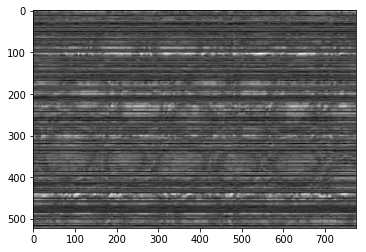
\includegraphics[width=0.45\textwidth]{Figures/CUR_col_100.png}\label{fig:sub3}}
\end{figure}

\begin{figure}[ht]
 \centering    
 \subfloat[Leverage score method]{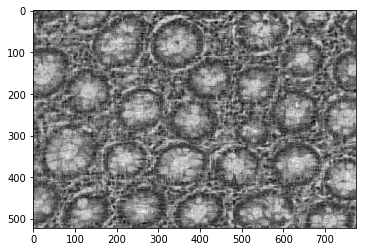
\includegraphics[width=0.45\textwidth]{Figures/CUR_lev_100.png}\label{fig:sub4}}
\end{figure}

\begin{figure}[ht]
 \centering    
 \subfloat[Block leverage score]{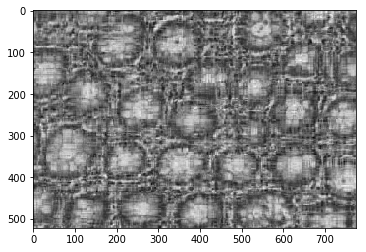
\includegraphics[width=0.45\textwidth]{Figures/Block_r12_87_129.png}\label{fig:sub5}}
\end{figure}



100 rows and columns sampled

\begin{tabular}{|c|c|c|c|c|c|c|} \hline
     Algorithms & Sampled & L2 norm & Nuclear norm& Frobenius norm & PSNR & Time taken\\ \hline
     CUR & 100,100 & 4.052 $\%$ & 46.4779$\%$ & 16.734 $\%$ & 21.202 & 0.4\\ \hline
     Linear time CUR & 100,100 & 87.67 $\%$ & 92.95$\%$ & 89.27 $\%$ & 6.316 & 0.4 \\ \hline
     Leverage score & 100,100& 3.35 $\%$ & 42.59$\%$ & 15 $\%$ & 21.80 & 0.4\\ \hline
     Block CUR($87 \times 129$) & 12,12 & 4.9579 $\%$ & 58.9837$\%$ & 20.6876 $\%$& 18.89 & 0.4\\ \hline
\end{tabular}

\begin{algorithm}[H]
\KwIn{ $A \in \mathbb{R}^{n \times d}, 1 \leq c \leq d, 1 \leq r \leq n, 1 \leq k \leq min(n,d)$}
\KwOut{$C \in \mathbb{R}^{n \times c}, U \in \mathbb{R}^{c \times r}, R \in \mathbb{R}^{r \times d}$}
\textbf{for} $t = \text{1 to c} $ \textbf{do}\;\\
    Pick $j \in \{1,...,d\}$ with probability $ p_{j} = ||A_{:,j}||^2/||A||^2_{F}$  (Modified to Cumulative Probability)\;\\
    Set $C_{:,t} = A_{:,j}/\sqrt{cp_{j}}$ \;
    
\textbf{for} $t = \text{1 to r} $ \textbf{do}\;\\
    Pick $i \in \{1,...,n\}$ with probability $ q_{i} = ||A_{i,:}||^2/||A||^2_{F}$ (Modified to Cumulative Probability)\; \\
    Set $R_{t,:} = A_{i,:}/\sqrt{rq_{i}}$ \; \\
    Set $\Psi_{:,t} = C_{i,:}/\sqrt{rq_{i}}$ \;
    
Set $k = min(k,rank(C^TC))$ \; 

Let $U = ([C^TC]_{k})^{-1} \Psi^T $ \;

\textbf{return} $C,U,R$ 
\caption{{\bf Linear Time CUR} \label{Algorithm}}
\end{algorithm}

\begin{algorithm}[H]
\KwIn{ $A \in \mathbb{R}^{n \times d}, 1 \leq c \leq d, 1 \leq r \leq n, 1 \leq k \leq min(n,d)$}
\KwOut{$C \in \mathbb{R}^{n \times c}, U \in \mathbb{R}^{c \times r}, R \in \mathbb{R}^{r \times d}$}
\textbf{for} $t = \text{1 to c} $ \textbf{do}\;\\
    Pick $j \in \{1,...,d\}$ with probability $ p_{j} = ||A_{:,j}||^2/||A||^2_{F}$  (Modified to Cumulative Probability)\;\\
    Set $C_{:,t} = A_{:,j}/\sqrt{cp_{j}}$ \;
    
\textbf{for} $t = \text{1 to r} $ \textbf{do}\;\\
    Pick $i \in \{1,...,n\}$ with probability $ q_{i} = ||A_{i,:}||^2/||A||^2_{F}$ (Modified to Cumulative Probability)\; \\
    Set $R_{t,:} = A_{i,:}/\sqrt{rq_{i}}$ \; \\

Let $U = C^{-1} X R^{-1}  $ \;

\textbf{return} $C,U,R$ 
\caption{{\bf CUR} \label{Algorithm cur}}
\end{algorithm}




\begin{algorithm}[H]
\KwIn{ $A \in \mathbb{R}^{n \times d}, 1 \leq c \leq d, 1 \leq k \leq min(n,d)$}
\KwOut{$C \in \mathbb{R}^{n \times c}$}

Compute svd of $A$ as $A = U\Sigma V^T$ and define normalized leverage scores as $p_i = \frac{1}{k}\Sigma^k_{j=1} V^2_{i,j} $

\textbf{for} $t = \text{1 to c} $ \textbf{do}\;\\
    Pick $j \in \{1,...,d\}$ with probability $ \min (1,c p_j)$ \;\\
    Set $C_{:,t} = A_{:,j}/\sqrt{c^2p_{j}}$ \;
    
\textbf{return} $C$ 
\caption{{\bf ColumnSelect} \label{Algorithm2}}
\end{algorithm}


\begin{algorithm}[h]
\KwIn{ $A \in \mathbb{R}^{n \times d}, 1 \leq c \leq d, 1 \leq r \leq n, 1 \leq k \leq min(n,d)$}
\KwOut{$C \in \mathbb{R}^{n \times c}, U \in \mathbb{R}^{c \times r}, R \in \mathbb{R}^{r \times d}$}
Run $ColumnSelect \text{ on } A \text{ with } c $ columns to construct the matrix $C$.

Run $ColumnSelect \text{ on } A^T \text{ with } r $  rows to construct the matrix $R$.

Set matrix $ U \text{ as } U = C^+AR^+ $ \; 

\textbf{return} $C,U,R$ 
\caption{{\bf LeverageScore CUR} \label{Algorithm3}}
\end{algorithm}

\begin{algorithm}[h]
\KwIn{ $A \in \mathbb{R}^{n \times d}, \text{no. of blocks} = p \times q, 1 \leq c \leq d/q, 1 \leq r \leq n/p$}
\KwOut{$ Blocks of C \in \mathbb{R}^{n/p \times c}, U \in \mathbb{R}^{c \times r}, R \in \mathbb{R}^{r \times d/q}$}

\textbf{for} $i = \text{1 to p} $ \textbf{do}\;\\
    \textbf{for} $j = \text{1 to q} $ \textbf{do}\;
    \quad Run CUR on the $block(i,j) = CUR$\\
\textbf{return} $C,U,R \text{ for each block }$ 
\caption{{\bf Block CUR} \label{Algorithm5}}
\end{algorithm}

% block wsi
% PSNR 22.97322269336675
% L2_norm error 0.5864106815066605%
% Nuclear_norm error 51.196954958313654%
% Frobenius_norm error 8.446171439043082%


In an attempt to speed up the process power SVD was tried but it was found out that inbuilt function is faster.

\subsection{Experiments on CUR}

Different number of rows and columns were sampled from the original image to construct C and R. (should try them again)

\begin{figure}[ht]
 \centering    
 \subfloat[Original WSI image]{\includegraphics[width=0.45\textwidth]{Figures/WSI_cropping.jpg}\label{fig:sub3}}
 
\end{figure}

\begin{figure} 
 \centering   
 \subfloat[4000 columns and 2000 rows sampled]{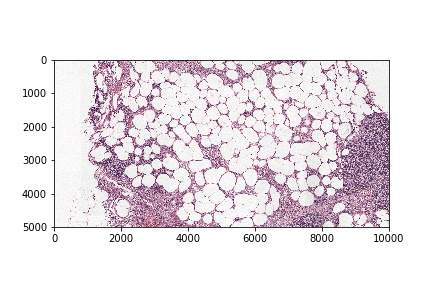
\includegraphics[width=0.55\textwidth]{Figures/CUR_4000c_2000r.jpg}\label{fig:sub3}}
 \hfill
 \subfloat[1000 columns and 100 rows sampled]{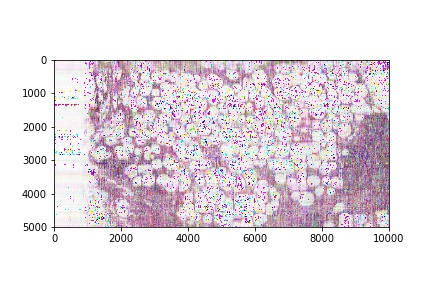
\includegraphics[width=0.55\textwidth]{Figures/CUR_1000c_100r.jpg}\label{fig:sub3}}
 \hfill
 \subfloat[40 columns and 20 rows sampled]{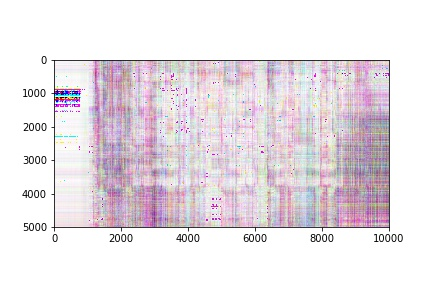
\includegraphics[width=0.55\textwidth]{Figures/CUR_40c_20r.jpg}\label{fig:sub3}}
 \caption{CUR decomposition}
\end{figure}




\section{Coherent Matrix Completion}
As we have discussed that there are different ways of doing CUR, in this section we discuss about the method based on leverage scores. It is shown that nuclear norm minimization can recover an arbitrary $n \times n$ matrix of rank r from $\mathcal{O}(nr\log^2{}n)$ revealed entries, provided that revealed entries are drawn proportionally to the local row and column coherences (closely related to leverage scores) of the underlying matrix.\cite{ChenCoherentCompletion}. 

Actually, the incoherence assumption is required because of the uniform sampling: coherent matrices are those which have most of their mass in a relatively small number of elements. By sampling entries uniformly and independently at random, most of the mass of a coherent low-rank matrix will be missed; this could (and does) throw off all existing recovery methods. One could imagine that if the sampling is dependent on the matrix, roughly in a way that elements with more mass are more likely to be observed, then it may be possible for existing methods to recover the full matrix.


The results in this paper hold for what is arguably the most popular approach to matrix completion: nuclear norm minimization. If the true matrix is $M$ with entries $M_{ij}$, and the
set of observed elements is $\Omega$, this method guesses as the
completion the optimum of the convex program
\begin{equation}
    \min_{X} ||X||_{*} 
    \text{   s.t   } X_{ij} = M_{ij} \text{  for } (i,j)  \in \Omega
\end{equation}

where the “nuclear norm” $||.||_{*}$ of a matrix is the sum of its
singular values. Throughout, we use the standard notation $f(n) = \Theta(g(n))$ to mean that $cg(n) \leq f(n) \leq Cg(n)$ for
some positive constants $c, C$, where $n := \max \{ n_1, n_2\}$.
We focus on the setting where matrix entries are revealed from an underlying probability distribution. To introduce the distribution of interest, we first need a definition
Chen et al.\cite{ChenCoherentCompletion}proposed two-phase sampling algorithm that can perform nearly as well as local-coherence sampling and without requiring a priori knowledge of the matrix coherence structure. In the experiments, we tried to implement it and run it on the example image.

\textbf{Definition 3.1.} For an $n1 \times n2$ real-valued matrix $M$ of
rank $r$ with SVD given by $U \Sigma V^T$ , the local coherences $ \mu_i$ for any row i, and $\nu_j$ for any column j - are defined by
the following relations
\begin{equation}
||U^Te_i|| = \sqrt{\frac{\mu_i r}{n_1}} , i = 1, . . . , n1
\end{equation}

\begin{equation}
    ||V^Te_j|| = \sqrt{\frac{\nu_j r}{n_2}} , j = 1, . . . , n1
\end{equation}

Note that the $\mu_i, \nu_j$s are non-negative, and since U and V
have orthonormal columns we always have $\Sigma_i \mu_i r/n_1 =
\Sigma_j \nu_j r/n_2  = r$

\textbf{Theorem 3.2.} Let $M = (M_{ij})$ be an $n_1 \times n_2$ matrix with local coherence parameters ${\mu_i,\nu_j}$, and suppose that its entries $M_{ij}$ are observed only over a subset of elements  $ \Omega \subseteq [n1] \times [n2]$. There are universal constants $c_0, c_1, c_2 >
0 $such that if each element (i, j) is independently observed
with probability $p_{ij}$, and $p_{ij}$ satisfies 
\begin{equation}
    p_ij \geq \min \{ c_0\frac{(\mu_i + \nu_j)rlog^2( n_1 + n_2)}{\min \{n_1, n_2\}}, 1 \}
\end{equation} 

\begin{equation}
    p_{ij} \geq \frac{1}{\min \{n_1,n_2\}^{10}} 
\end{equation}
 

then M is the unique optimal solution to the nuclear norm minimization problem (1) with probability at least $1-c_1(n_1 + n_2)^{-c_2}$

%Finally, we apply our results to quantify how weighted nuclear norm minimization can improve on unweighted minimization given an arbitrary set of sampled entries.


For matrix completion, Singular Value Thresholding algorithm was used.\cite{CaiACOMPLETION}

\textbf{Singular Value Thresholding}
write more about that algorithm



\begin{algorithm}[ht]
\KwIn{ Sampled matrix $P_{\Omega}(M)$, rank parameter $r$, and $m,\beta$ such that $|\Omega| = \beta m $  }
\KwOut{Completed Matrix $\hat{M}$}

Compute the rank-$r$ SVD of   $P_{\Omega} (M), \hat{U} \hat{\Sigma} \hat{V}^T  $

Estimate the local coherences by $\hat{\mu_{i}} = \frac{n_1}{r}||\hat{U}^Te_i||^2 $
and $\hat{\nu_{i}} = \frac{n_2}{r}||\hat{V}^Te_j||^2 $

Generate a set of $(1-\beta)m$ new samples $\Bar{\Omega}$ distributed as $ \Bar{p}_{ij} = \min \{ c_0 \frac{(\mu_i + \nu_j)r log^2(n_1 + n_2)}{min(n_1,n_2)}, 1  \} $ (Modified to cumulative probability)

$ \hat{M} = \arg \min ||X||_{*} \text{ s.t } P_{\Omega \cup \Bar{\Omega}} (X) = P_{\Omega \cup \Bar{\Omega}} (M) $ \;

\textbf{return} $\hat{M}$ 
\caption{{\bf Two phase Coherency based sampling} \label{Algorithm two}}
\end{algorithm}


\subsection{Experiments on Sampling based on Coherency}
Before trying two-phase sampling, we tried first local-coherence sampling. Rank was chosen based on SNR value around 20 and sampling was kept constant at 25 percent. Both ways were tried, one rank for all 3 bands and different ranks for different bands. Ranks 100 and 60 were tried in the case for one rank for all 3 bands. These ranks were chosen based on SNR for the grayscale image.
\begin{figure}[ht]
 \centering  
 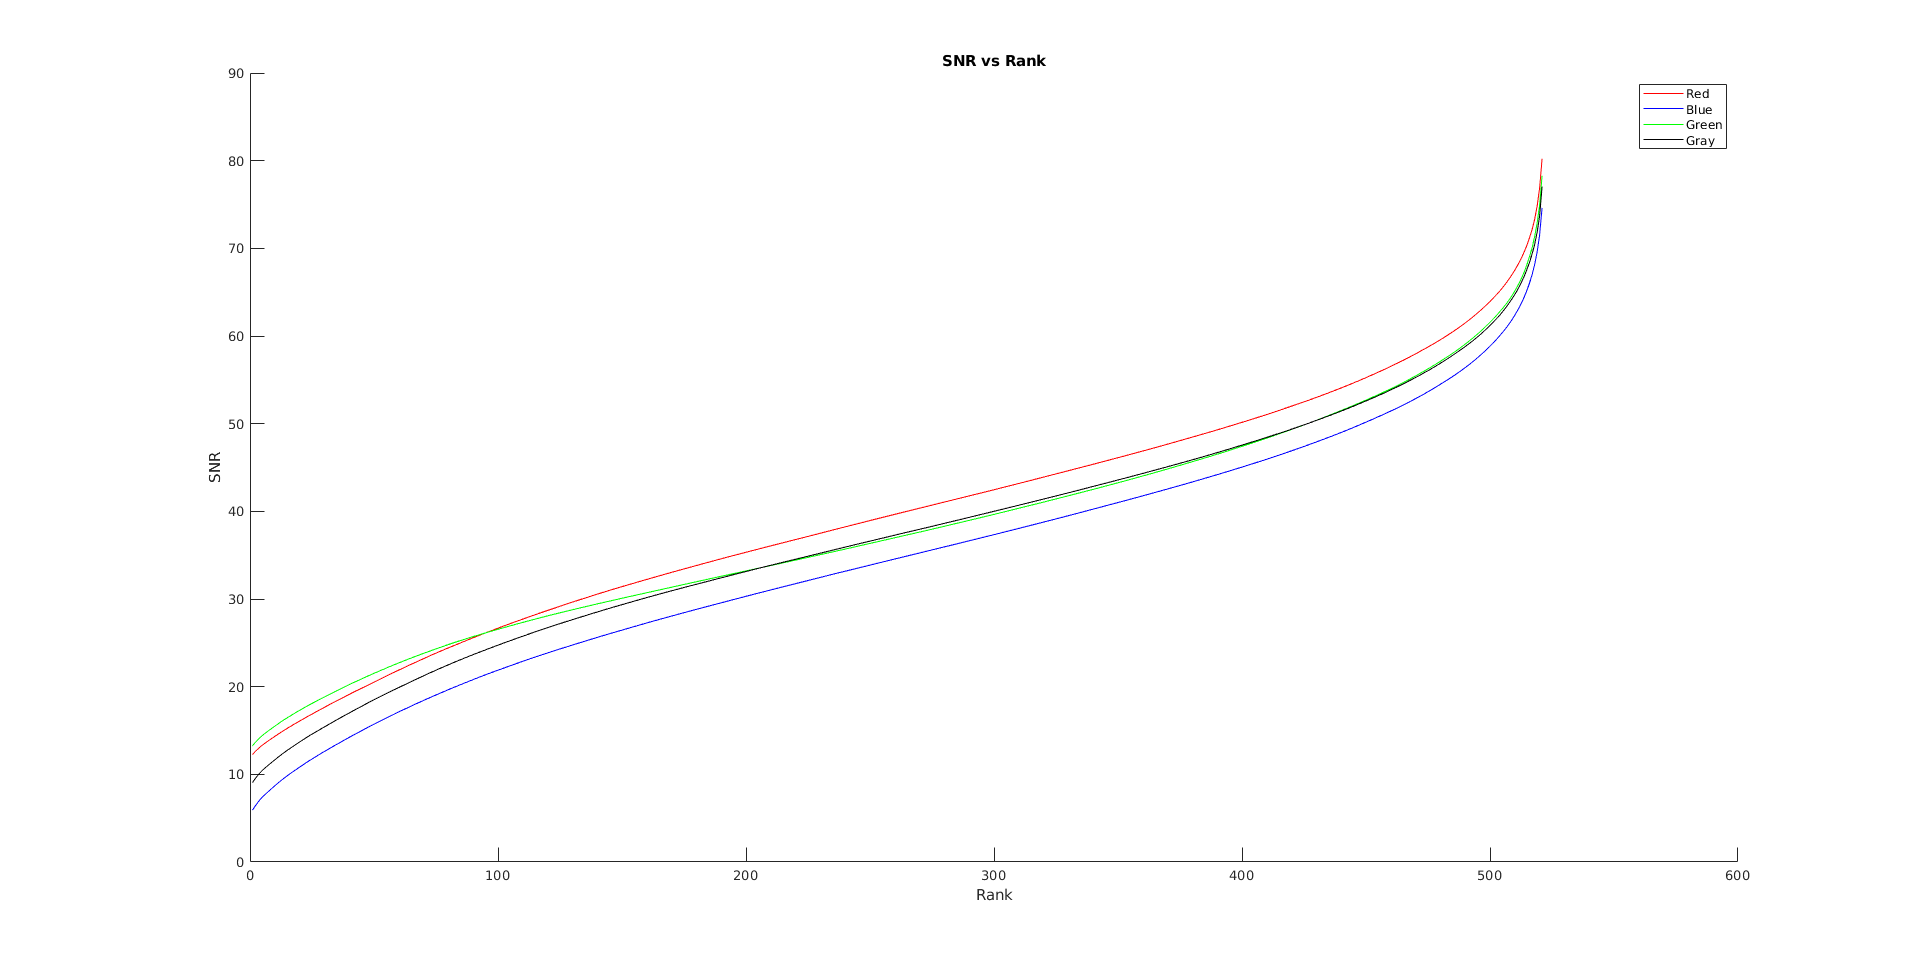
\includegraphics[width=0.9\textwidth]{Figures/SNR.png}
 \label{fig:1}
 \caption{SNR for chosing ranks}
\end{figure} 
\begin{figure}[ht]
 \centering  
 \subfloat[Original image]{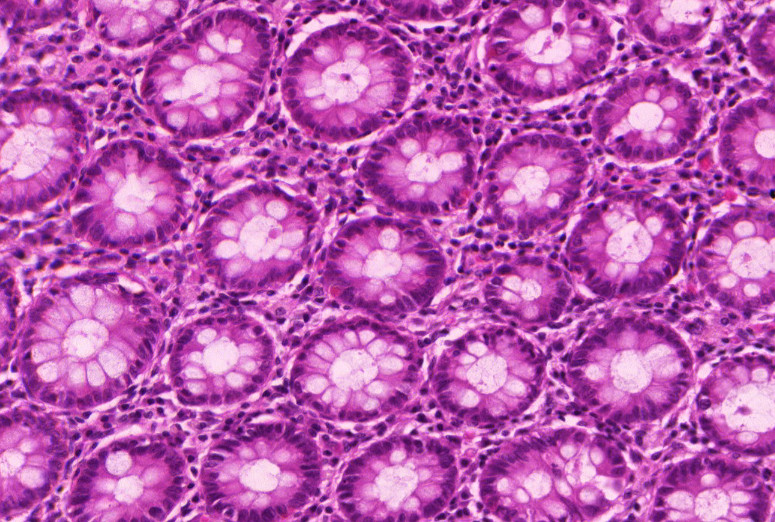
\includegraphics[width=0.35\textwidth]{Figures/10-12813-01-2.jpg}\label{fig:sub1}}
 \hfill
 \subfloat[Rank 100 image PSNR = 19.8678, SSIM =   0.8816
]{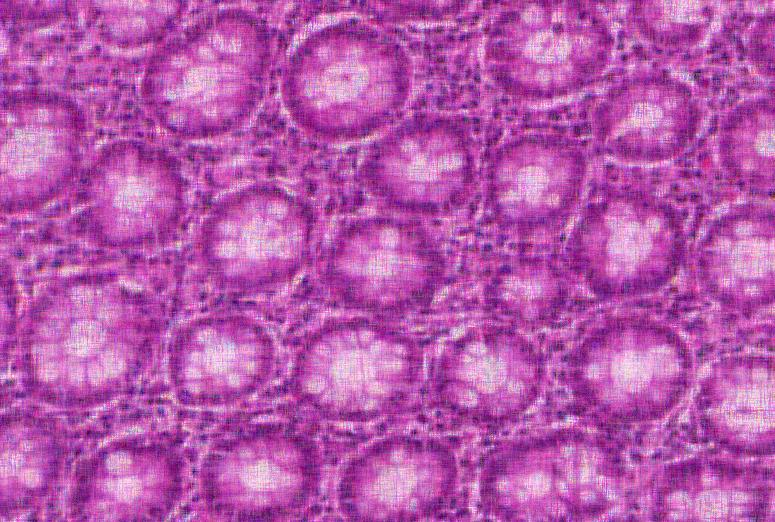
\includegraphics[width=0.35\textwidth]{Figures/output_100.jpg}\label{fig:sub2}}
 \caption{Coherent matrix completion example}
\end{figure} 

\begin{figure}[ht]
 \centering    
 \subfloat[Rank 60 image PSNR = 20.7961, SSIM =  0.8983
]{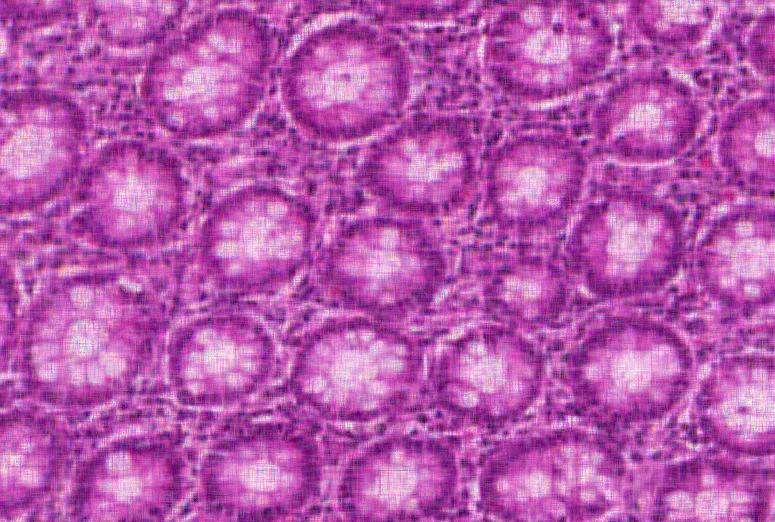
\includegraphics[width=0.35\textwidth]{Figures/output_60.jpg}\label{fig:sub3}}
 \hfill
 \subfloat[Different Rank PSNR = 20.6481, SSIM = 0.8914]{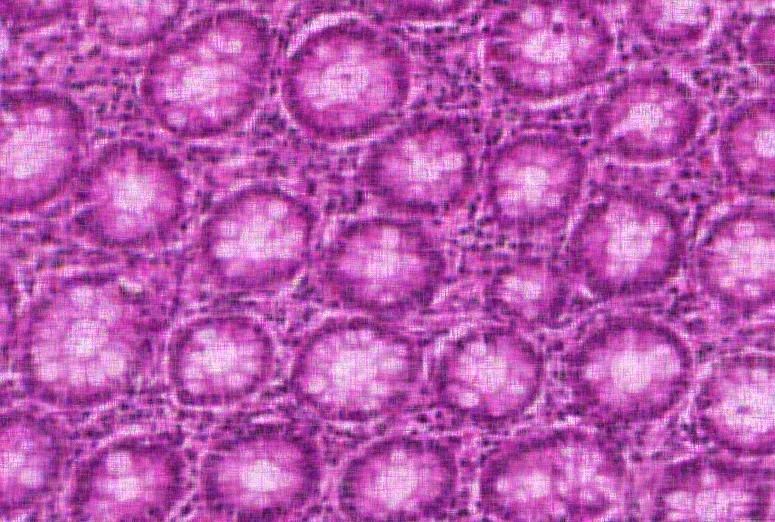
\includegraphics[width=0.35\textwidth]{Figures/output_diff_rank.jpg}\label{fig:sub3}}
 \caption{Coherent matrix completion example}
\end{figure}


To compare this with random sampling, random sampling was also tried for the same image.

\begin{figure}[ht]
 \centering    
 \subfloat[Original image]{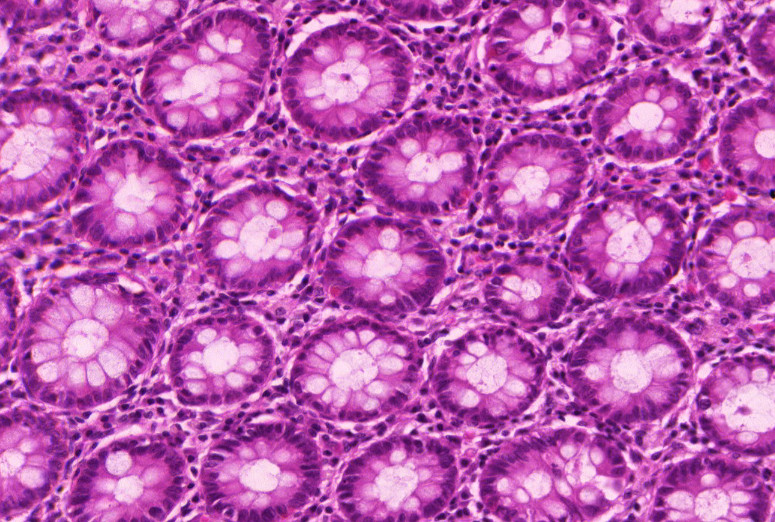
\includegraphics[width=0.35\textwidth]{Figures/10-12813-01-2.jpg}\label{fig:sub3}}
 \hfill
 \subfloat[Coherency based Sampling PSNR = 20.7961, SSIM =  0.8983]{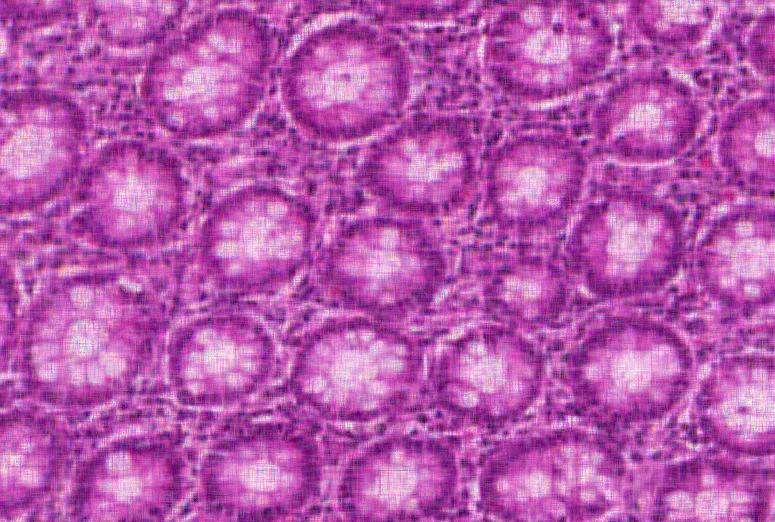
\includegraphics[width=0.35\textwidth]{Figures/output_60.jpg}\label{fig:sub3}}
 \hfill
 \subfloat[Random Sampling PSNR =  21.8035,  SSIM = 0.9139
]{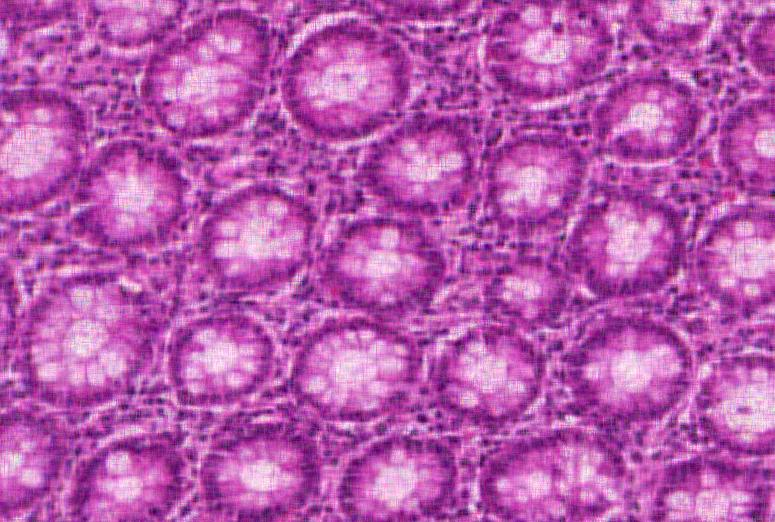
\includegraphics[width=0.35\textwidth]{Figures/random_output_60.jpg}\label{fig:sub3}}
 \caption{Coherent matrix sampling vs Random matrix sampling}
\end{figure}



For bigger image of size $1000 \times 1000$, this was done using Patches of size $250 \times 250$.  

\begin{figure}[ht]
 \centering    
 \subfloat[Original WSI image]{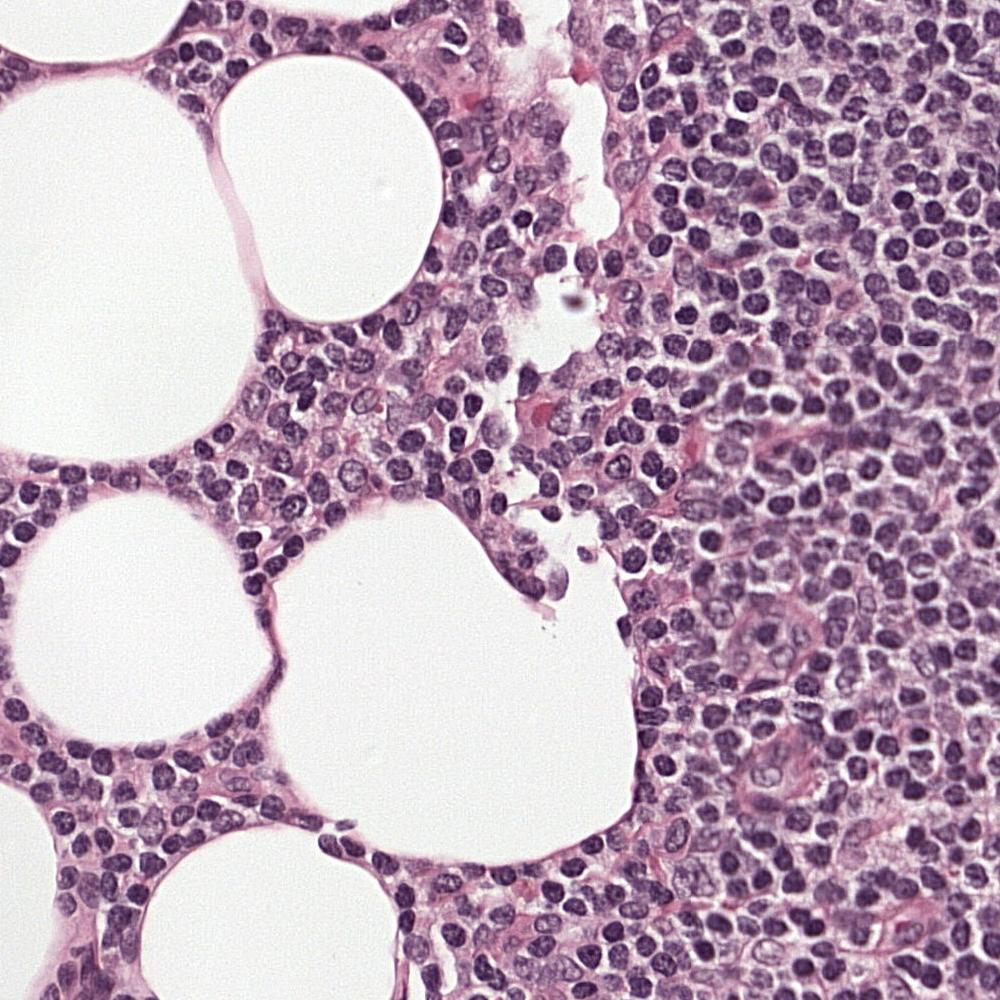
\includegraphics[width=0.35\textwidth]{Figures/WSI_cropped_1000.jpg}\label{fig:sub3}}
 \hfill
 \subfloat[Reconstructed WSI image in patchwise manner SSIM = 0.7356, PSNR=21.5107]{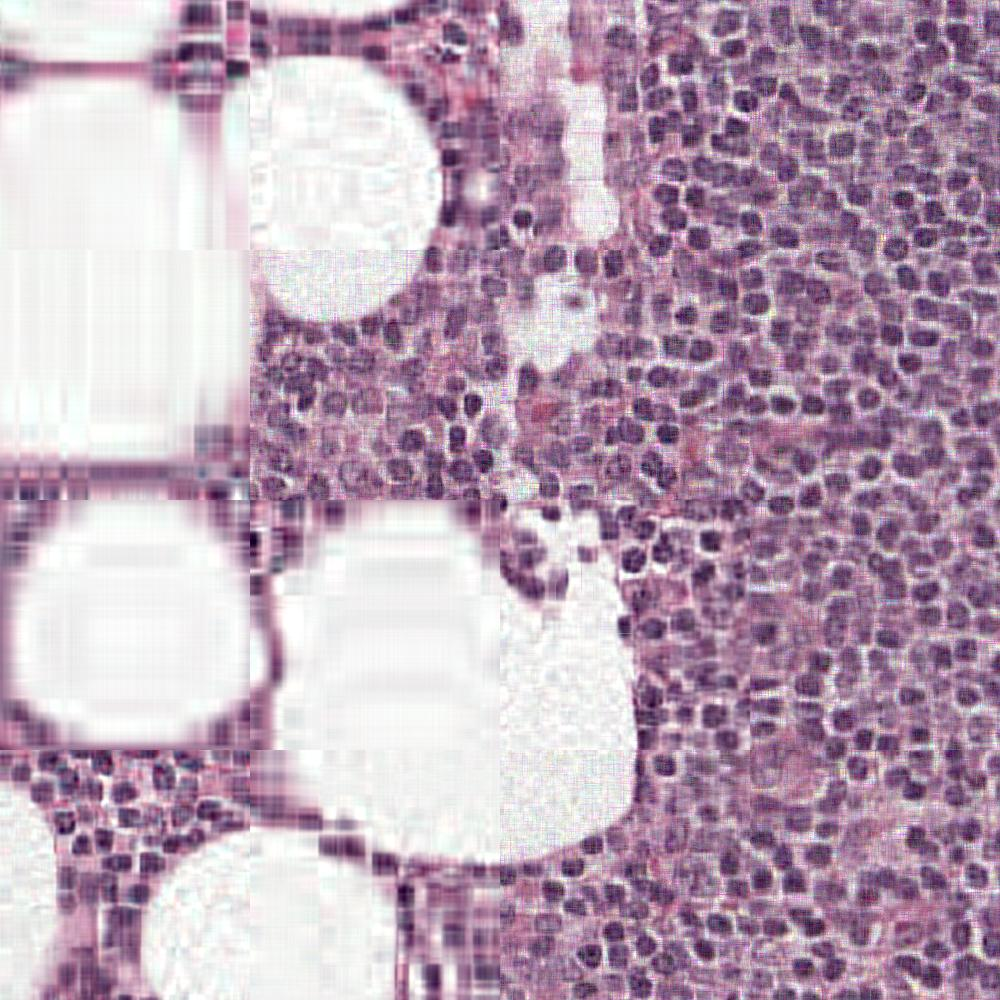
\includegraphics[width=0.35\textwidth]{Figures/WSI_mat_com_1000.jpg}\label{fig:sub3}}
 \caption{Patchwise Coherent matrix completion example}
\end{figure}

When two phase sampling was tried, it diverged. 


\section{Asymptotic Structure in Compressed Sensing}
Principles like asymptotic incoherence, asymptotic sparsity and multilevel sampling are utilized by Roman et al for compressive sensing.\cite{Roman2014OnSensing}  This new theory says optimal sampling depends on the structure of the signal and the resolution.


A traditional CS setup is as follows. The aim is to recover a signal $f$ from an incomplete (subsampled) set of measurements $y$. Here,
$f$ is represented as a vector in $\mathbb{C}^N$ and is assumed to be $s$-sparse in
some orthonormal basis $\Phi \in \mathbb{C}^{N \times N}$ (e.g. wavelets) called \textit{sparsity
basis.} This means that its vector of coefficients $x = \Phi f$ has at most $s$ nonzero entries. Let $\Psi \in \mathbb{C}^{N \times N}$ be an orthonormal basis, called
\textit{sensing or sampling basis}, and write $U = \Psi \Phi^* = (u_{ij})$, which is an 
isometry. The coherence of $U$ is

$$ \mu(U) = \max_{i,j}|u_{ij}|^2 \in [1/N,1]$$

and $U$ is said to be perfectly incoherent if $\mu(U) = 1/N $

Let the \textit{subsampling pattern} be the set $\Omega \subseteq {1,...,N}$ of cardinality $m$ with its elements chosen uniformly at random. Owing to a result by Candes and Plan (4) and Adcock and Hansen (5), if we have access to the subset of measurements $y = P_{\Omega} \Psi f$ then $f$ can be
recovered from y exactly with probability at least $1 - \epsilon$ if
$$m \gtrsim \mu(U ) \cdot N \cdot s \cdot (1 + log(1/\epsilon )) \cdot log(N)$$
 
where $P_{\Omega} \in \{0,1\}^{N \times N}$ is the diagonal projection matrix with the $j^{th}$ entry 1 if $j \in \Omega$ and 0 otherwise, and the notation $a \gtrsim b$ means that $a \geq Cb$ where $C>0$ is some constant independent of a and b. Then, $f$ is recovered by solving

%$$ \min_{z \in \mathbb{C}^N}||z||_1 \text{ subject to } ||y-P_{\Omega}Uz|| \leq \eta$$

\begin{equation}%\label{eq:3}
    \min_{z \in \mathbb{C}^N}||z||_1 \text{ subject to } ||y-P_{\Omega}Uz|| \leq \eta
\end{equation}
\\
where $\eta$ is chosen according to the noise level (0 if noiseless). \\
\\
\textbf{The real world is often coherent.} The root cause of this lack of incoherence is the discretization of what is intrinsically an infinite-dimensional problem into a finite-dimensional one. In short, U converges to an infinite matrix (3) and since the incoherence is the supremum of its entries, there exists some N for which a coherence barrier is hit, resulting in the worst case for a CS recovery. Changing $\Psi$ may provide marginal benefits, if any, since the coherence barrier always occurs at some N .\\
\\
\textbf{Sparsity, flip test and the absence of RIP.} Flip test allows one to evaluate whether sampling strategy is completely independent of the location of the non-zero coefficients of an s-sparse vector $x$, i.e. with the $s$ nonzero coefficients at arbitrary locations. Let $x \in \mathbb{C}^N$ be a vector, and $U \in \mathbb{C}^{N\times N}$ a measurement matrix. We then sample according to some pattern $\Omega \subseteq \{1,..,N\} \text{ with } |\Omega|= m$ and solve Eq. for $x$, i.e. $min||z||_1 \text{ s.t } P_{\Omega} Uz=P_{\Omega}Ux$ to obtain a reconstruction $z= \alpha.$ Now we flip $x$ to obtain a vector $x^{'}$ with reverse entries, $x^{'}_{i} = x_{N-1}, i= 1,...,N$ and solve for $x^{'}$ using the same $U$ and $\Omega$, i.e. $min||z||_1 \text{ s.t } P_{\Omega} Uz=P_{\Omega}Ux^{'}$.  Assuming $z$ to be a solution, then by flipping $z$ we obtain a second reconstruction $\alpha$ of the original vector $x$, where $\alpha_i = z_{N-i}$.
\\
Assume $\Omega$ is a sampling pattern for recovering $x$ using $\alpha$. If sparsity alone dictates the reconstruction quality, then $\alpha$ must yield the same reconstruction quality (since x has the same sparsity as x, being merely a permutation of x). As is evident, the flipped recovery $\alpha$ is substantially worse than its unflipped version $\alpha'$. This confirms that sparsity alone does not dictate
the reconstruction quality. Furthermore, note that $ P_{\Omega} U$ cannot satisfy an RIP for realistic values of N , m and s. 

\subsection{Asymptotic sparsity}
Besides being sparse, practical  signals have more structure, namely asymptotic sparsity, i.e. they are far sparser at fine scales (large  k) than at coarse scales (small k). This also holds for other function  systems such as curvelets, contourlets, or shearlets.

\begin{figure}[ht]
 \centering    
 \subfloat[Original image]{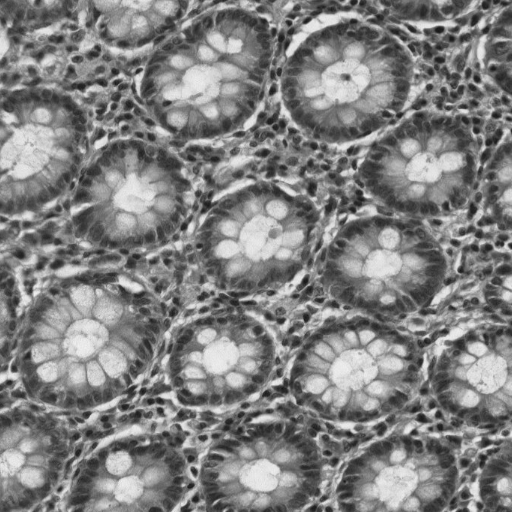
\includegraphics[width=0.35\textwidth]{Figures/tubule_512.png}\label{fig:sub3}}
 \hfill
 \subfloat[Local Sparsity]{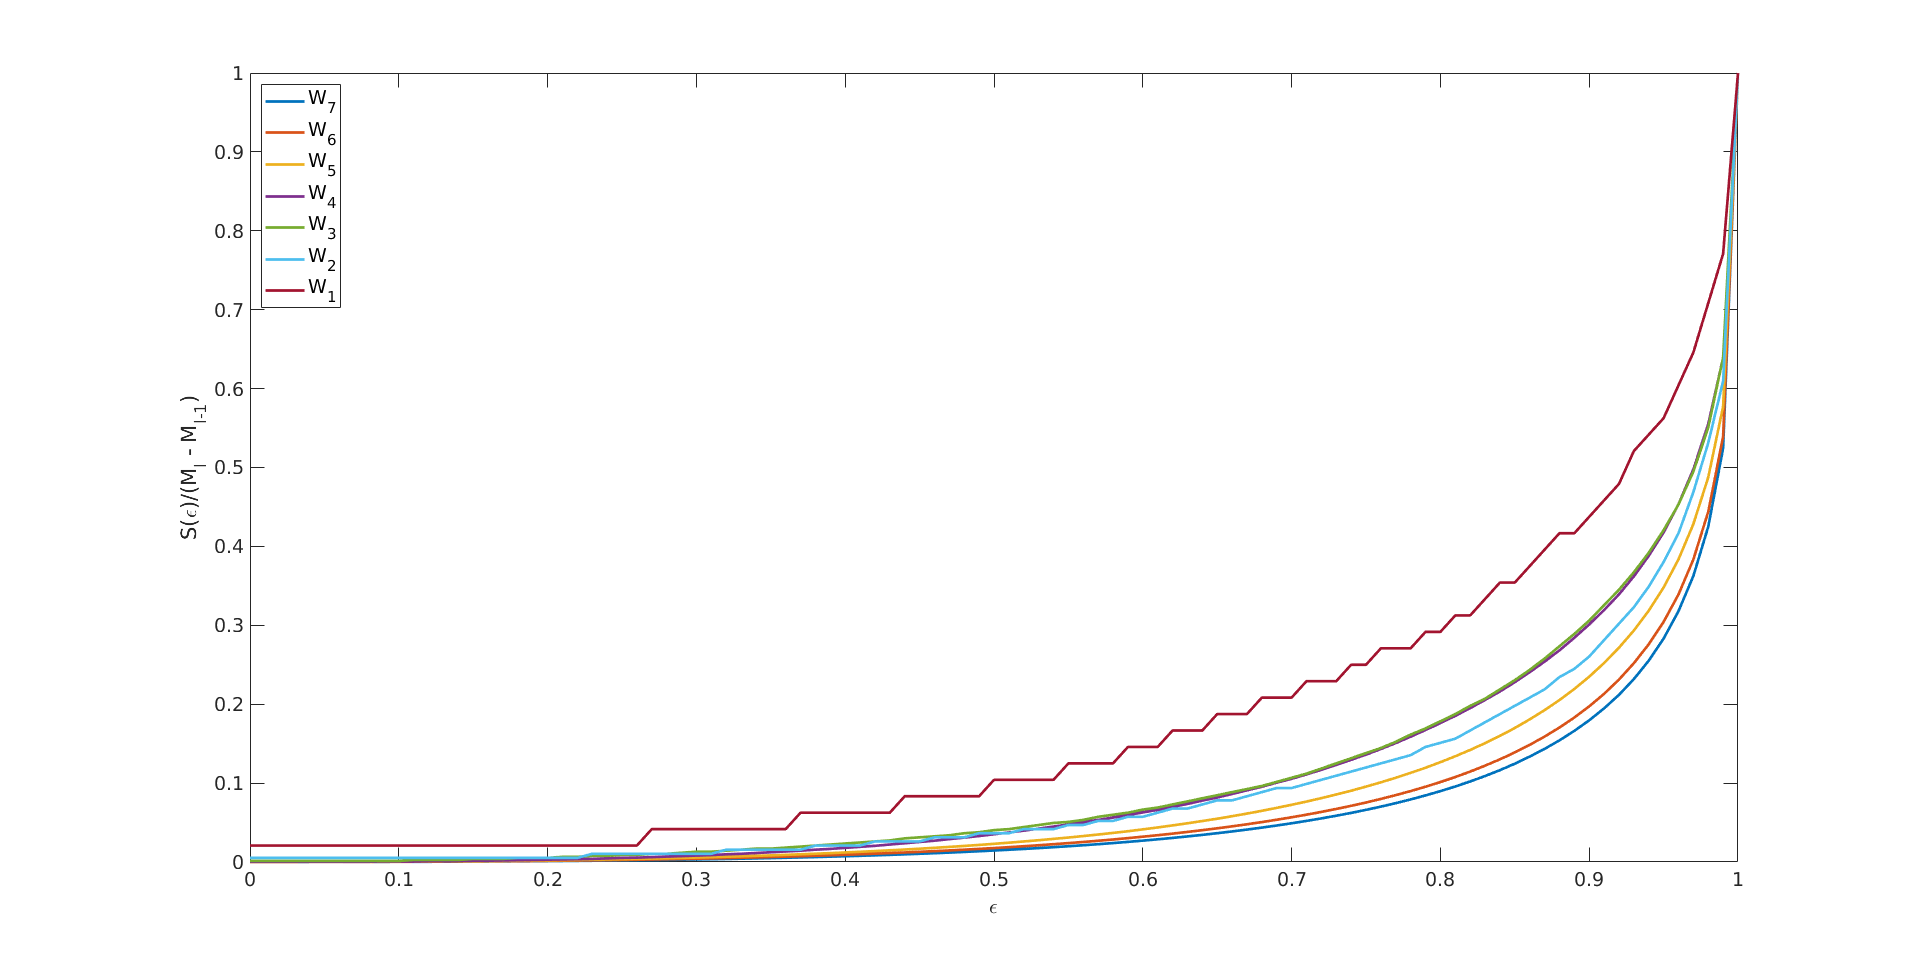
\includegraphics[width=0.75\textwidth]{Figures/local_sparsity.png}\label{fig:sub3}}
 \caption{Asymptotic sparsity}
\end{figure}


\subsection{Asymptotic incoherence}
In contrast with random matrices (e.g.Gaussian or Bernoulli), many sampling and sparsifying operators typically found in practice yield fully coherent problems.  In brief, U is asymptotically incoherent if the coherences of the matrices formed by removing either the first K rows or columns of U are small. 


\begin{figure}[ht]
 \centering  
 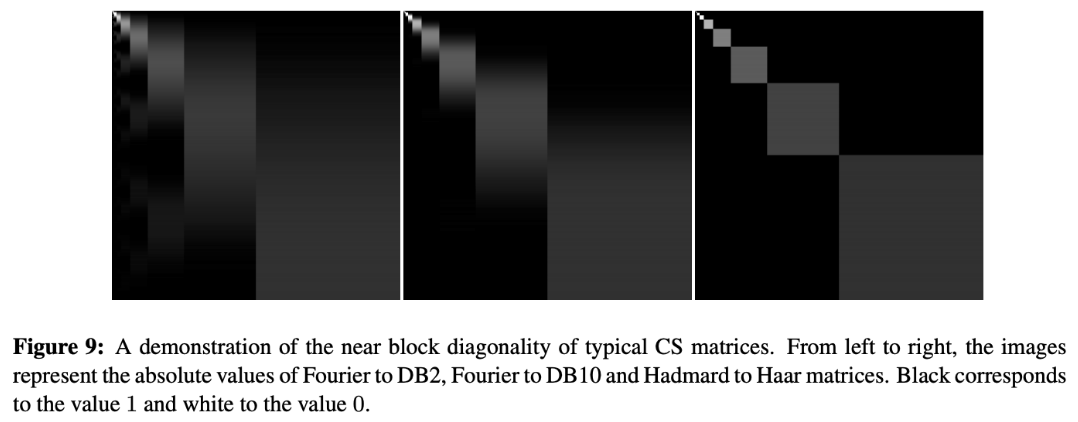
\includegraphics[width=0.75\textwidth]{Figures/Incoherence.png}
 \label{fig:1}
 \caption{Asymptotic incoherence}
\end{figure}


\subsection{Multilevel sampling}
Asymptotic incoherence calls for a different strategy than uniform random sampling. High coherence in the first few rows of U means that important information about the signal to be recovered is likely to be contained in the corresponding measurements, and thus we should fully sample these rows. Once outside this region, as coherence starts decreasing, we can subsample gradually.

Flexible all-round multilevel sampling scheme was devised in this paper\cite{Roman2014OnSensing}. Assuming the coefficients $f \in C^{N \times N}$ of a sampling orthonormal basis, e.g. DFT, our multilevel sampling scheme divides $f$ into $n$ regions delimited by $n-1$ equispaced concentric circles plus the full square. Normalizing the support of f to $[-1,1]^2$, the circles have radius $r_k$
with $k = 0,... , n-1$, which are given by $r_0 = m$ and $r_k = k \cdot \frac{1-m}{n-1}$
for $k > 0$, where $m \in (0,1)$ is a parameter. In each of the $n$ regions,
the fraction of coefficients sampled with uniform probability is
$$p_k = exp(-(bk/n)^a)$$ 
where $k = 0, ... , n$ and $a > 0$ and $b > 0$ are parameters. The total fraction of subsampled coefficients is $p = \sum_{k}p_k A_k$, where $A_k$ is
the normalized area of the $k^{th}$ region. Since $p_0 = 1$ and $p_k > p_{k+1}$,
the first region will sample all coefficients and the remaining regions will sample a decreasing fraction.


\subsection{Effects and benefits of the new principles}
\textbf{ The optimal sampling strategy is signal dependent.} As the flip test shows, the optimal sampling strategy depends on the structure of  the signal. Multilevel sampling takes this into account and allows one  to further improve the CS recovery by tailoring the sampling according to e.g. the resolution and expected wavelet structure of the signal. This has additional advantages as one can mitigate application-specific hurdles or target application-specific features (e.g. brain and  spine imaging would use different subsampling schemes). An important effect is that regardless of the sampling basis and subsampling scheme, the quality of the reconstruction increases as resolution increases. This is first revealed by fixing the subsampling strategy and fraction across resolutions, and a more striking result is obtained by fixing the number (instead of fraction) of samples, revealing hidden details, previously inaccessible. This is due to signals being typically increasingly (asymptotically) sparse at higher resolutions. 

 \textbf{Resolution dependency.} An important effect is that regardless of  the sampling basis and subsampling scheme, the quality of the reconstruction increases as resolution increases. This is first revealed by fixing the subsampling strategy and fraction across resolutions, and a more striking result is obtained by fixing the number (instead of fraction) of samples, revealing hidden details, previously inaccessible. This is due to signals being typically increasingly (asymptotically)
sparse at higher resolutions. 
 \textbf{Infinite dimensional CS}. The errors arising from recovering the continuous samples using discrete models are sometimes significant (9). The section Infinite dimensional problems discusses this aspect and shows an EM
 example where such noticeable errors can be overcome by using generalized sampling theory (3) and recovery into boundary wavelets.
 
\textbf{Structured sampling vs Structured Recovery.} We exploit sparsity structure by using multilevel sampling of asymptotically incoherent matrices and standard minimization algorithms. Alternatively, sparsity structure can be exploited by using universal sampling matrices (e.g. random Gaussian/Bernoulli) and modified recovery algorithms. The advantages of the former, which, in contrast with the latter, allows to choose
the sparsity frame, is applicable to both Type I and Type II problems, and yields overall superior results.

\textbf{Structure vs Universality:Asymptotic vs Uniform incoherence.}
The Structure vs Universality section argues that universal matrices offer little room to exploit extra structure the signal may have, even in Type II problems, and that non-universal matrices, such as Hadamard, coupled with multilevel sampling provide a better solution for both Type I and Type II problems as they can exploit the prevalent asymptotic sparsity of signals in practice.

\textbf{Storage and speed.} Random matrices are slow and require (large) storage. This yields slow recovery and limits the maximum signal size, which severely affects computations and, more importantly, sparsity structure. The Storage/speed section discusses this aspect and also shows that simply addressing the speed and storage problems via fast transforms and non-random matrices is not sufficient to achieve improved recovery compared to what multilevel sampling of non-universal matrices can offer.


\subsection{Wavelet}

\subsection{Hadamard}

% \subsection{Fourier}

% \cite{antun2016coherence}


\subsection{Experiments}

Traditionally the compressive sensing theory have been focusing on the three principles of sparsity, incoherence and uniform random subsampling. Recent years research have shown that these principles yield insufficient results in many
practical setups. This has lead to the development of the principles of asymptotic sparsity, asymptotic incoherence and multilevel random subsampling.

As a result of these principles, the current theory is limited to unitary sampling and sparsifying operators. For large scale reconstruction, the theory is further restricted to operators whose product can be computed in $O(N log_2 N)$ operations, due to memory constraints of computers. Accordingly this has increased the popularity of the Fourier and Hadamard sampling operators, for applications where these operators can model the underlying sampling structure. As the sparsifying operator the wavelet transform have proven to yield satisfactory results in most setups. Since all of these operators needs to be unitary, this have restricted us to only consider Daubechies compactly supported orthonormal wavelets. By using wavelets as the sparsifying transform it has been proven that a Fourier sampling basis will be asymptotically incoherent to a unitary wavelet basis. The same result can easily be calculated numerically between a Hadamard sampling basis and a Daubechies wavelet basis. However, any theoretical result
of this fact have been lacking. The purpose of this text is to provide such a
theoretical result


We used following algorithm for doing Multi-level sampling

\begin{algorithm}[h]
\KwIn{ $A \in \mathbb{R}^{n \times d}, \text{no. of samples for sampling } M = const \times m, \text{no. of samples for sparse approximation } m = percent \times n \times d, \text{Choose the sparsifying and measurement system}, level \in \{1,2,.. \} $ }

\KwOut{$ \text{ Restored } D \in \mathbb{R}^{n \times d}$}
\text{B = Spare Approximation(A,level,percent)}

\text{Indices = Multi-level-sampling(n,d,level,percent)}

\text{C = Recovery in sparse domain(A,B,Indices,level)}

\text{D = Convert to original domain(C)}

\textbf{return} $D$ 
\caption{{\bf Multi-level sampling} \label{Algorithm multi-level}}
\end{algorithm}



The solver used was SPGL1: A solver for large-scale sparse reconstruction.\cite{spgl1:2007}. This solver solves the basis pursuit denoise. Basis  pursuit  denoise.The basis pursuit problem aims to find a sparse solution of the underdetermined system of equations $Ax=b$, where $A$ is an $m \times n$ matrix and b is an $m$-vector.  Typically,$m << n$, and the problem is ill-posed.  The approach advocated by Chen et al. [15] is to solve the convex optimization problem(BP)

    % minimizex‖x‖1subject toAx=b.
\begin{equation}
\min ||x||_1 \text{ subject to } Ax = b 
\end{equation}

In the presence of noisy or imperfect data, however, it is undesirable to exactly fit the linear system. Instead, the constraint in (BP) is relaxed to obtain the basis pursuit denoise (BPDN) problem(BP-$\sigma$)
\begin{equation}
%minimizex‖x‖1subject to‖Ax−b‖2≤σ,
\min ||x||_1 \text{ subject to } ||Ax-b||_2\leq  \sigma
\end{equation}

where the positive parameter $\sigma$ is an estimate of the noise level in the data.  The case $\sigma = 0$ corresponds to a solution of (BP)-i.e., a basis pursuit solution

\textbf{Spectral projected gradient $\ell_1$  algorithm}

\begin{equation}
%minimize ||Ax ´ b||2 subject to ||x||1 ⁄ τ: (LSτ)
\min ||x||_1 \text{ subject to } ||Ax-b||_2 \leq \eta  \text{              }     (P_1,{\eta})  
\end{equation}

Recovery of large signals using convex optimization software will often be constrained by memory limitations on computers. Thus, if the signal is large enough, it will simply be impractical to store the sampling and sparsifying
operators as matrices. To overcome this difficulty, we have indicated that we will apply linear operators on $\mathbb{C}^N$ which can be computed in-place using $O (N log_2 N)$ operations. One challenge with this approach is that most conic solvers require a densely stored matrix to solve $(P_1, \eta)$, making it impossible to bypass the memory bottle-neck.

An algorithm which handles these issue is the spectral projected gradient $\ell_1$  (SPG$\ell_1$) algorithm [5, 7]. This algorithm works iteratively, by only using operations which require the matrices $A$ and $A^T$ to be linear operators. Hence, it does not involve any computations of the pseudo-inverse, as required by most of the algorithms above. This enables us to save enormous amounts of memory, by using matrices whose products can be computed in-place.
The SPG$\ell_1$ algorithm tries to solve the $(P_1, \eta)$ problem for a fixed $\eta \in [0,||b||_2]$
by finding a sequence of solutions to an equivalent problem formulation [21, prop. 3.2]. This equivalent formulation is often denoted the least absolute shrinkage and selection operator (LASSO), and uses a one-norm constraint. That is 
\begin{equation}
%minimize ||Ax ´ b||2 subject to ||x||1 ⁄ τ: (LSτ)
\min ||Ax-b||_2 \text{ subject to } ||x||_1 \leq \tau  \text{   }     (LS_{\tau})  
\end{equation}

As both of these formulations fall into the category of vector optimization
problems with no unique optimal value, any solution of either one of them will
be Pareto optimal [8, Sec. 4.7.3]. A general problem with these formulations is
that it is impossible to know a priori for what values of $\eta$ and $\tau$ these solutions
coincide.
Next, let $x_{\tau}$ be a solution of $(LS_{\tau})$ and let $\tau_{\eta}$ denote the value of $\tau$ for which the solution of $(P_1; \eta)$and $(LS_{\tau})$ coincide. In [5] it was proved that the
optimal solutions of  $(LS_{\tau})$  for all values of $\tau \in [0,\tau_{\eta}]$ defines a continuously differentiable curve. As all points along this curve is Pareto optimal it is
denote as the Pareto curve. It was further proven that for $\tau \in [0,\tau_{\eta}] $;  the single
parameter function

\begin{equation}
    \phi (\tau) = ||r_{\tau}||_2 \text{ with } r_ {\tau}:= b - Ax_{\tau}   
\end{equation}
was strictly decreasing. One was also able to find an explicit expression for its
derivative using the solution $x_{\tau}$ of $(LS_{\tau})$,
\begin{equation}
    \phi^{`} (\tau) = -||\frac{A^T r_{\tau}}{||r_{\tau}||_2}||_{\infty}
\end{equation}

In total, this enable us to use a Newton-based root-finding algorithm to find
the final solution $\phi(\tau) = \eta $. Hence, start by setting $\tau_{0} = 0 $ and solve $(LS \tau)$.
This gives us a solution $x_{\tau0}$. Next, evaluate $\nabla \tau_0$ for this
$x_{\tau_0}$ and compute $\tau_1 = \tau_0 + \nabla \tau_0$. Repeat this process until $\phi(\tau) = \eta $.

For this algorithm to work, a critical requirement is to solve the $(LS\tau)$
problem in an efficient manner. This is done by the spectral projected-gradient (SPG) algorithm. This algorithm consists of two potentially costly operations. First, one need to implement an efficients projection operator
\begin{equation}
    P_{\tau}(c) :={ \arg \min ||c-x||_{2} \text{ subject to } ||x||_1 \leq \tau } 
\end{equation}

to project any vector onto the feasible set $\{x: ||x||_1 \leq \tau \}$. This can be done
using at most $O(Nlog_2N)$ operations by following an algorithm given in [5].

The second critical step is to compute the gradient of the function $f(x) = \frac{1}{2}||Ax-b||^2_2$
i.e., . The matrix-vector products found
in this gradient could potentially have a cost of $O(N^2)$, but with our use of
operators we know that it can be computed using only $O(N log_2 N)$ operations.
As a result, both of the potentially expensive operations can be computed
efficiently.

The idea of the SPG algorithm is to start with an initial solution $x_0$ and
search for a new solution along the gradient $\nabla  f(x_0)$. This is done by choosing
a step length $\alpha$ and compute a new solution $x_1 = P_{\tau}(x_0 - \alpha \nabla f(x_0) ) $. This
process is then repeated until some stopping criterion is met.
% There are more technicalities concerning this algorithm, which have been
% omitted here. Interested readers are referred to [5] for the mathematical details, while the authors C++ implementation can be found online for technical
% details. In figure 2.3 we have compared this implementation with the default
% Matlab package [6]. As we can see from the figure, both of these implementations yield sufficient results, but the computational time of the former is higher.
% All other figures in this text have therefore been computed with the Matlab
% algorithm

\subsubsection{Changing percentage and Changing Constant} 
As we increase the percentage or constant (Remember  $M = const \times perc \times n_1 \times n_2$ ), total number of samples increase so the recovery is better. After few trials, $per = 3 \%$ and $const = 6$ was fixed for rest of the experiments as total samples are around $20 \%$.

\subsubsection{Changing Levels}

At first, Hadamard and Haar wavelet combination was tried with different levels. After level 3, there is not much significant improvement in PSNR.

\begin{figure}[ht]
 \centering    
 \subfloat[Level 1 (PSNR 6.89) ]{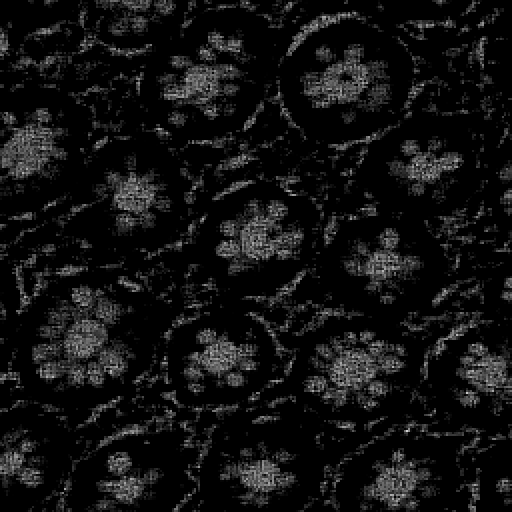
\includegraphics[width=0.35\textwidth]{Figures/level1.png}\label{fig:sub 12}}
 \hfill
 \subfloat[Level 2 (PSNR 11.2) ]{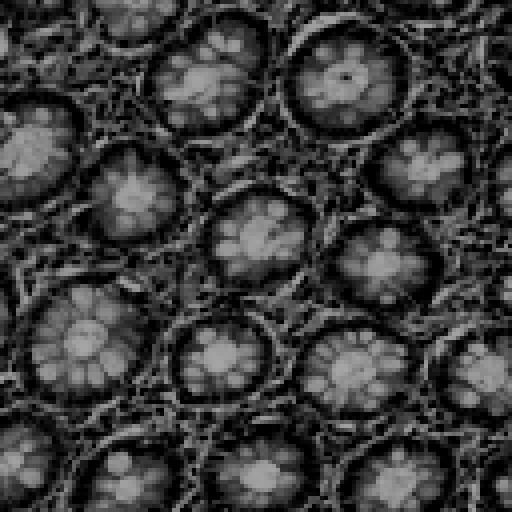
\includegraphics[width=0.35\textwidth]{Figures/level2.png}\label{fig:sub 13}}
 \hfill
 \subfloat[Level 5 (PSNR 21.94) ]{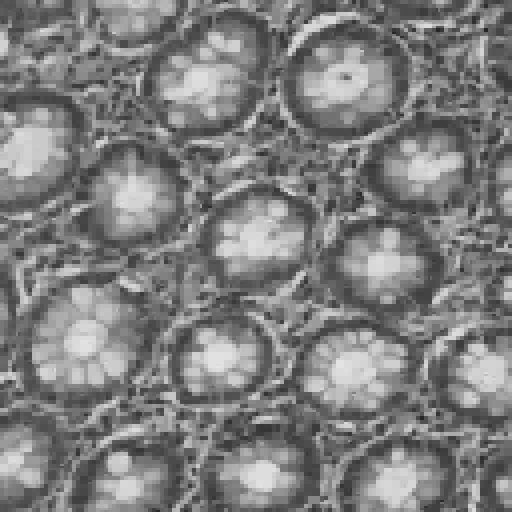
\includegraphics[width=0.35\textwidth]{Figures/level5.png}\label{fig:sub 14}}
 \hfill
 \subfloat[Level 8 (PSNR 21.95) ]{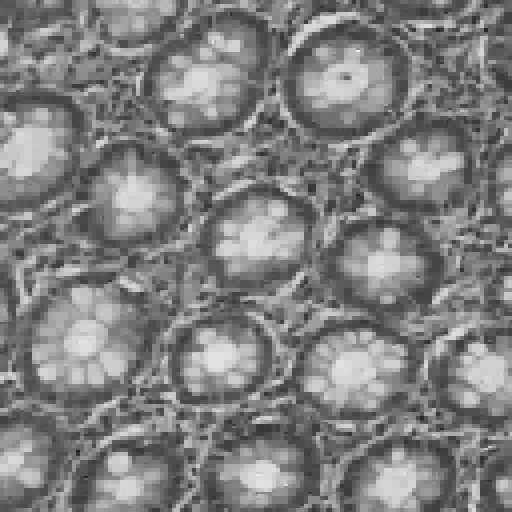
\includegraphics[width=0.35\textwidth]{Figures/level8.png}\label{fig:sub 15}}
 \caption{Various levels of multi-level sampling}
\end{figure}


\begin{figure}[ht]
 \centering    
 \subfloat[PSNR]{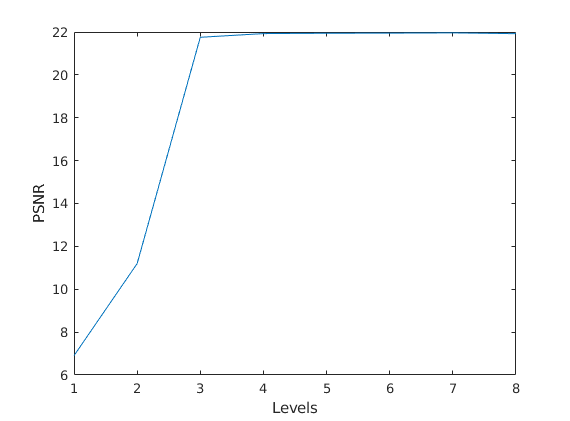
\includegraphics[width=0.35\textwidth]{Figures/psnr.png}\label{fig:sub 22}}
 \hfill
 \subfloat[2-Norm error]{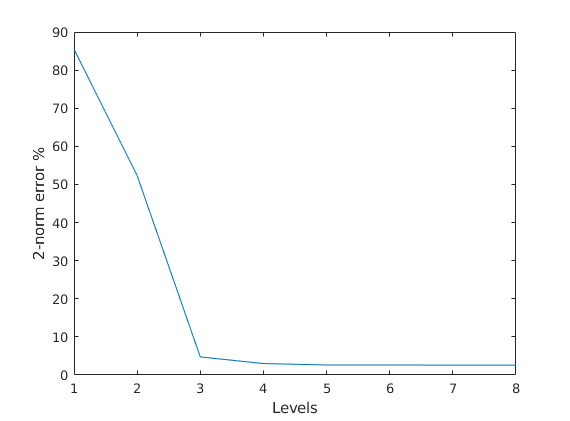
\includegraphics[width=0.35\textwidth]{Figures/2norm.png}\label{fig:sub 23}}
 \hfill
 \subfloat[Inf-norm error]{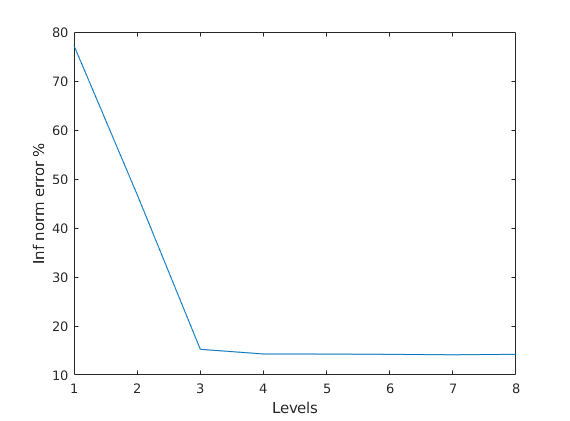
\includegraphics[width=0.35\textwidth]{Figures/infnorm.png}\label{fig:sub 24}}
 \hfill
 \subfloat[Frobenius norm]{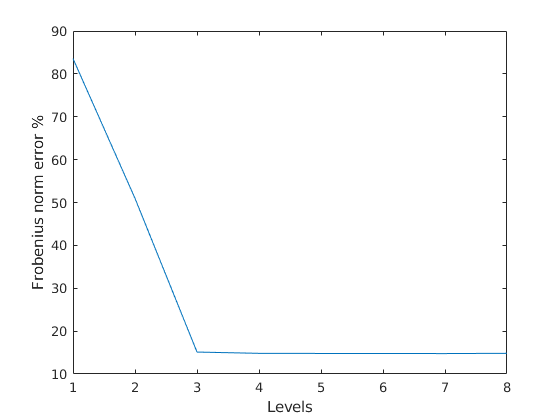
\includegraphics[width=0.35\textwidth]{Figures/fronorm.png}\label{fig:sub 25}}
 \caption{Various levels of multi-level sampling}
\end{figure}


\subsubsection{Changing Sparsifying and Measurement system}

Now keeping the level fixed, we change sparsifying and measurement system. We can see that DB2 and Hadamard gives the best result. 


\cite{adcock2015quest}
\begin{figure}[h]
 \centering    
%  \subfloat[Random  (PSNR 18.08)]{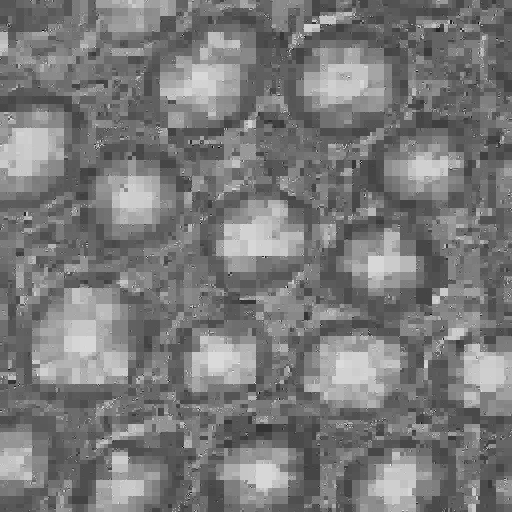
\includegraphics[width=0.35\textwidth]{Figures/random.png}\label{fig:sub 32}}
%  \hfill
 \subfloat[Fourier and Haar  (PSNR 16.43) ]{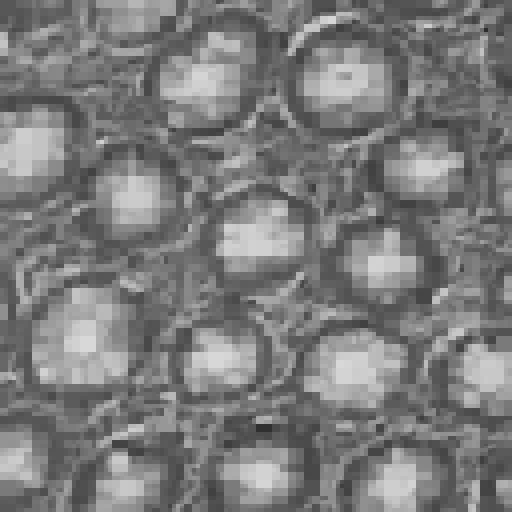
\includegraphics[width=0.35\textwidth]{Figures/fourier_haar.png}\label{fig:sub 33}}
 \hfill
 \subfloat[Fourier and DB2  (PSNR 10.90) ]{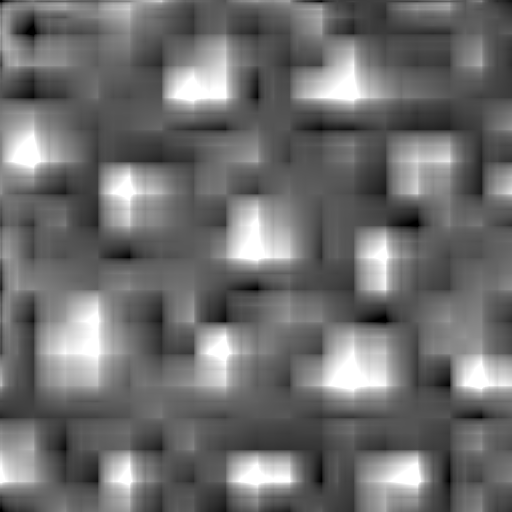
\includegraphics[width=0.35\textwidth]{Figures/fourier_db2.png}\label{fig:sub 34}}
 \hfill
 \subfloat[Hadamard and Haar (PSNR 21.93) ]{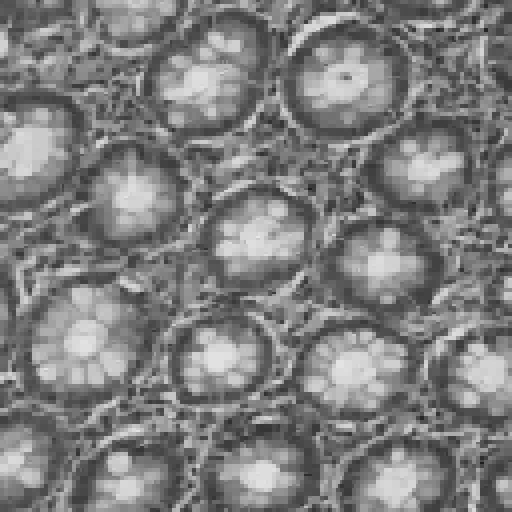
\includegraphics[width=0.35\textwidth]{Figures/hadamard_haar.png}\label{fig:sub 35}}
 \hfill
 \subfloat[Hadamard and DB2  (PSNR 23.39)]{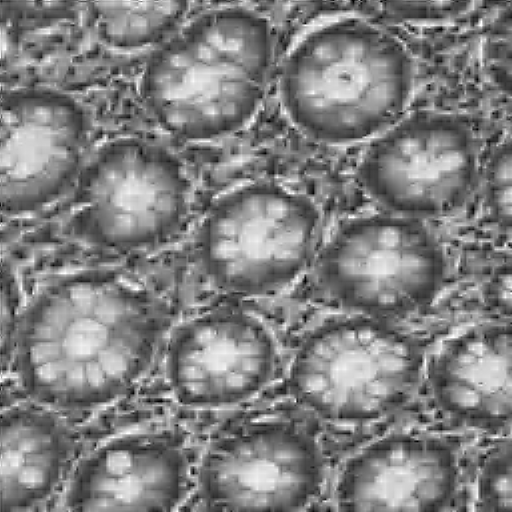
\includegraphics[width=0.35\textwidth]{Figures/hadamard_db2.png}\label{fig:sub 35}}
 \caption{Different combinations}
\end{figure}

\begin{figure}[h]
 \centering    
 \subfloat[Random  (PSNR 18.08)]{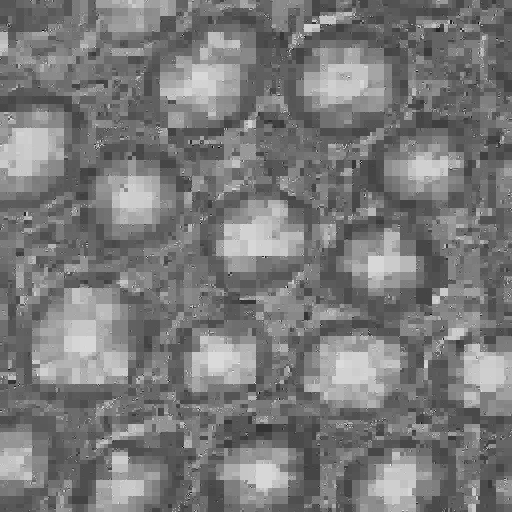
\includegraphics[width=0.35\textwidth]{Figures/random.png}\label{fig:sub 32}}
 \caption{Different combinations}
\end{figure} 


\subsection{Progressive Sampling}

We know that sampling scheme tries to sample from each level in round robin fashion. When we want 20\% samples, we get following number of samples in each level. 

\begin{figure}[ht]
 \centering  
 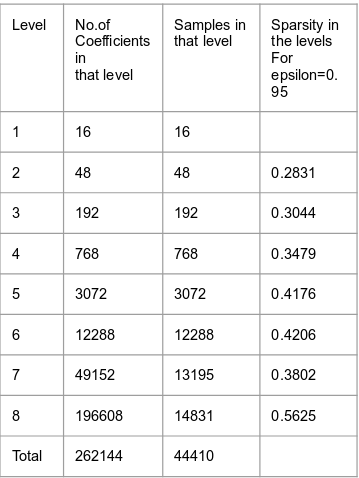
\includegraphics[width=0.25\textwidth]{Figures/Sample_each_level.png}
 \label{fig:1}
 \caption{Samples at each level}
\end{figure}

Now we would like to see how the reconstructed image becomes as we consider samples at different levels progressively.

\begin{figure}[ht]
 \centering  
 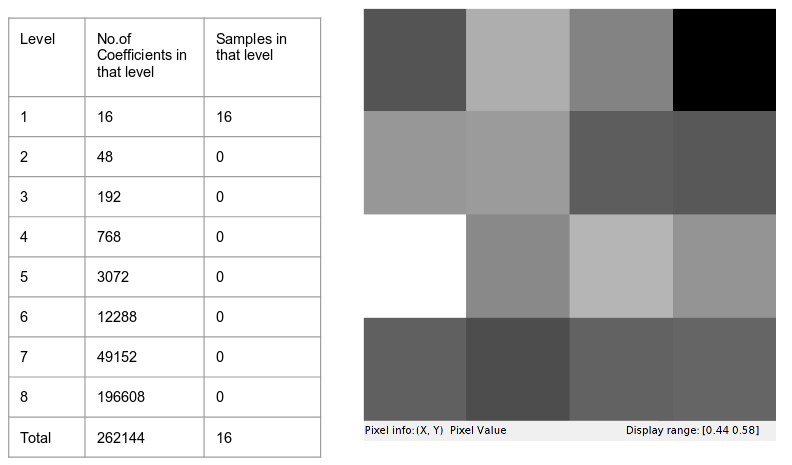
\includegraphics[width=0.75\textwidth]{Figures/upto_level1.png}
 \label{fig:1}
 \caption{Samples upto level 1}
\end{figure}


\begin{figure}[ht]
 \centering  
 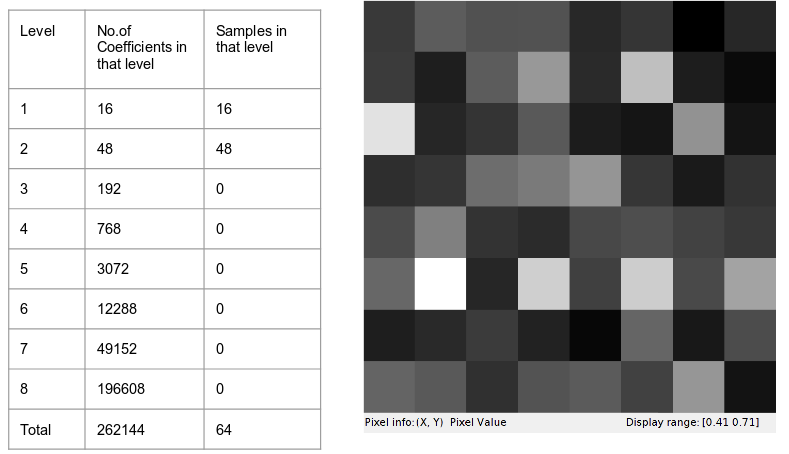
\includegraphics[width=0.75\textwidth]{Figures/upto_level2.png}
 \label{fig:1}
 \caption{Samples upto level 2}
\end{figure}


\begin{figure}[ht]
 \centering  
 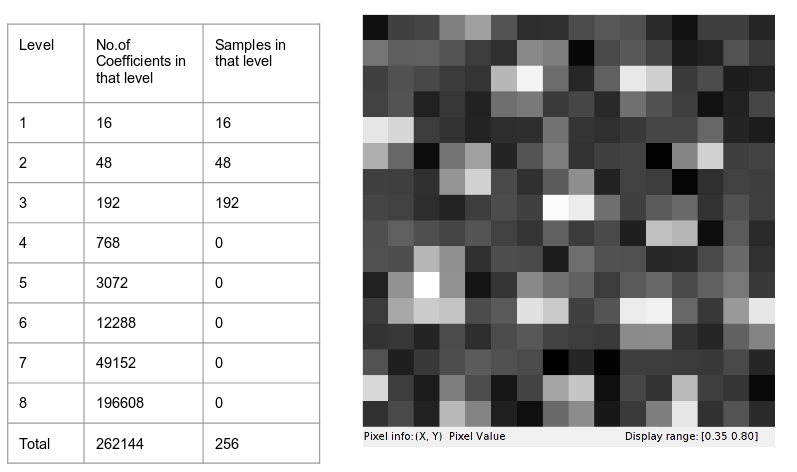
\includegraphics[width=0.75\textwidth]{Figures/upto_level3.png}
 \label{fig:1}
 \caption{Samples upto level 3}
\end{figure}

\begin{figure}[ht]
 \centering  
 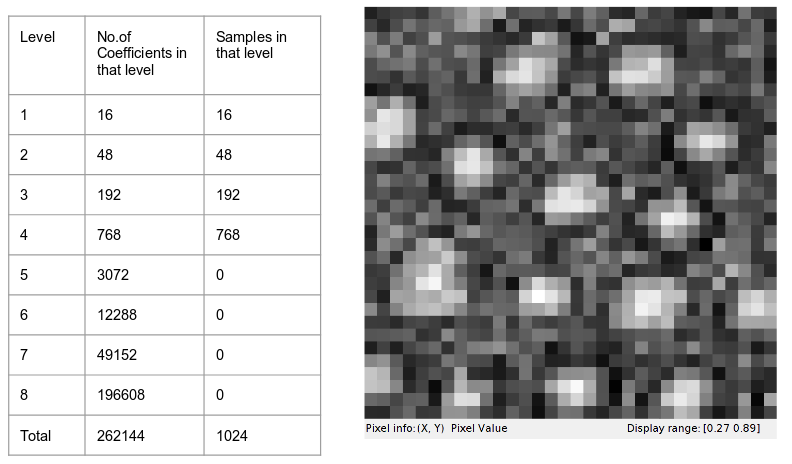
\includegraphics[width=0.75\textwidth]{Figures/upto_level4.png}
 \label{fig:1}
 \caption{Samples upto level 4}
\end{figure}

\begin{figure}[ht]
 \centering  
 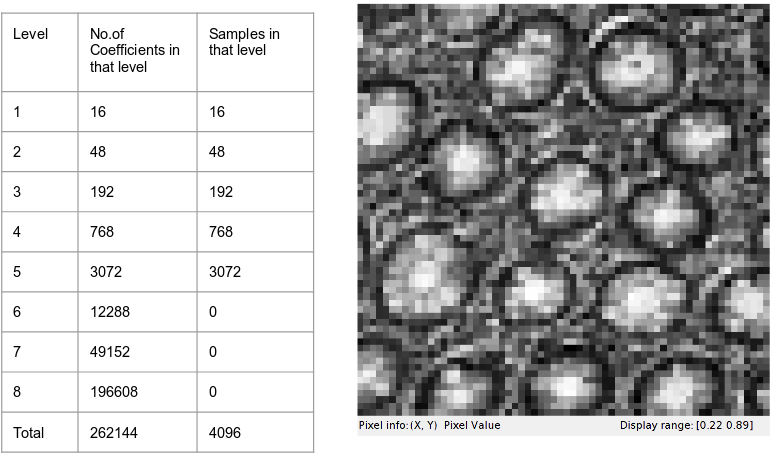
\includegraphics[width=0.75\textwidth]{Figures/upto_level5.png}
 \label{fig:1}
 \caption{Samples upto level 5}
\end{figure}

\begin{figure}[ht]
 \centering  
 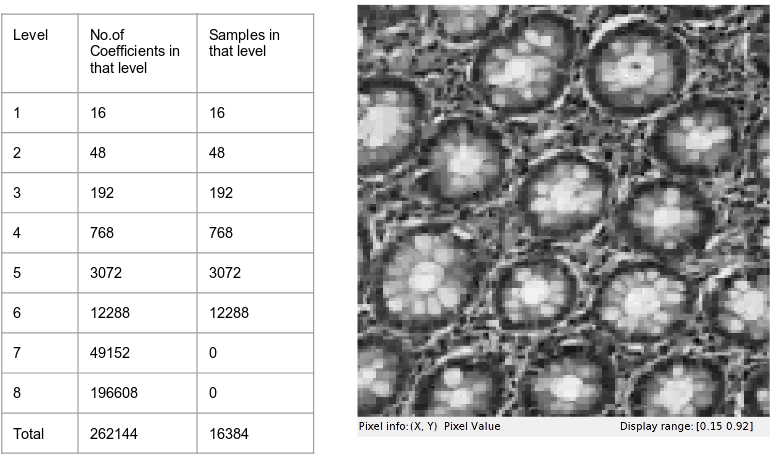
\includegraphics[width=0.75\textwidth]{Figures/upto_level6.png}
 \label{fig:1}
 \caption{Samples upto level 6}
\end{figure}

\begin{figure}[ht]
 \centering  
 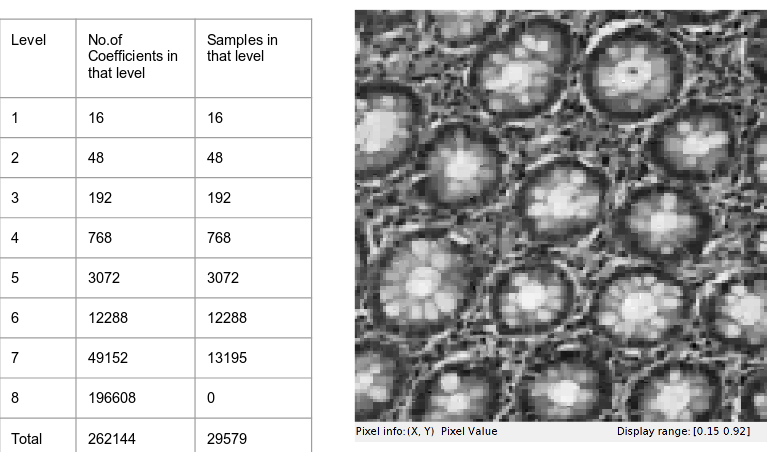
\includegraphics[width=0.75\textwidth]{Figures/upto_level7.png}
 \label{fig:1}
 \caption{Samples upto level 7}
\end{figure}

\begin{figure}[ht]
 \centering  
 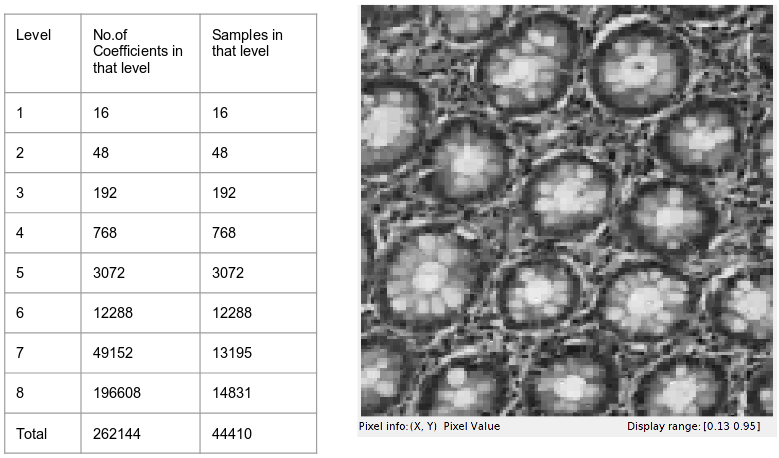
\includegraphics[width=0.75\textwidth]{Figures/upto_level8.png}
 \label{fig:1}
 \caption{Samples upto level 8}
\end{figure}


\begin{figure}[ht]
 \centering  
 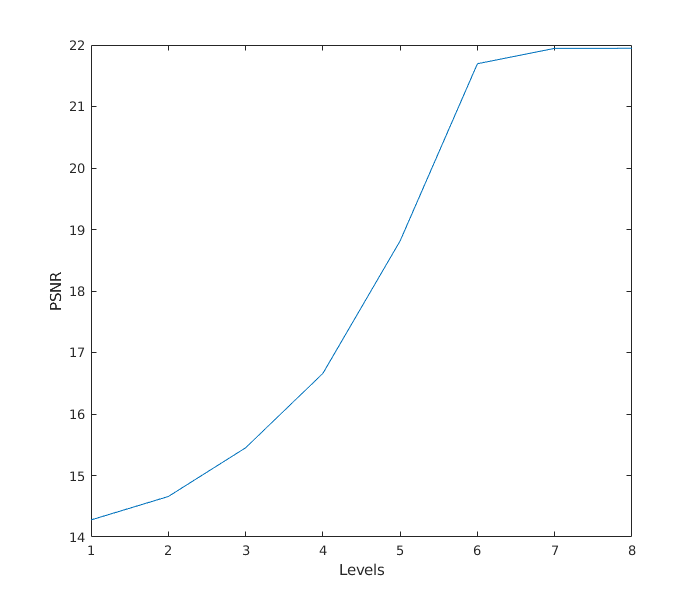
\includegraphics[width=0.5\textwidth]{Figures/psnr_sampling.png}
 \label{fig:1}
 \caption{PSNR vs levels}
\end{figure}

As we can see, as we consider samples from different levels, reconstruction becomes better and better. Notice that, all the coefficients were sampled upto 6 levels. It is also surprising that even though we sampled few points in level 8, there was not significant increase in PSNR.

If I put those many number of samples in level 7, I get PSNR of 22.1823, which is more than 21.9464 which we get according to samples in all 8 levels.

To understand the sampling scheme better we focus on whether the sampling scheme i.e no.of samples in each level is related to sparsity at that level or not. We see that it is not the case so we should try to sample accordingly.








% \subsubsection{Two-phase with Multi-level}

% Two-phase sampling was tried using different combinations with coherency sampling. So we do random or multi-level sampling first and using those we do coherency based sampling. We sampled $M =0.03*3$ at each phase.

% \begin{tabular}{|c|c|c|c|c|c|c|} \hline
%      First phase & L2 norm & Infinity norm & Frobenius norm & PSNR & Time taken\\ \hline
%      Random & 6.75 $\%$ & 23.69$\%$ & 23.6955 $\%$ & 17.88 & 1.213378e+02 \\ \hline
%      Fourier+Haar & 52.38 $\%$ & 92.27$\%$ & 94.78 $\%$ & 5.816 &  1.254187e+02  \\ \hline
%      Hadamard+Haar & 3.52 $\%$ & 18.91$\%$ & 18.33 $\%$ & 20.0313 & 1.220593e+02s\\ \hline
     
% \end{tabular}




















% Second, it demonstrates that the optimal sampling strategy and the efficiency of compressed sensing also depends on the resolution of the problem, and shows how this phenomenon markedly affects compressed sensing results and how to exploit it. Third, as the new framework also fits analog (infinite dimensional) models that govern many inverse problems in practice, the paper describes how it can be used to yield substantial improvements. Fourth, by using multilevel sampling, which exploits the structure of the signal, the paper explains how one can outperform random Gaussian/Bernoulli sampling even when the classical l1 recovery algorithm is replaced by modified algorithms which aim to exploit structure such as model based or Bayesian compressed sensing or approximate message passaging. 

% \section{Tensor Sketching}
% Till now we have discussed various matrix based methods, now we will discuss about tensor methods. Like in Matrices we have SVD for calculating low rank approximation, for Tensor we have two ways for calculating tensor approximations. One is CP and other is Tucker Decomposition. We will be discussing those methods in detail. 
 
% \subsection{CP Decomposition}
% Write what it is and the algorithm \cite{Rabanser2017IntroductionLearning}

% \subsection{Tucker Decomposition}
% Write what it is and the algorithm


% In this discuss about this paper\cite{Xia2017EffectiveSparsification}



% \section{Fast and Accurate Low Rank Factorization of Compressively-Sensed Data}

% We consider the question of accurately and efficiently computing low-rank matrix or tensor factorizations given data compressed via random projections. This
% problem arises naturally in the many settings in which data is acquired via compressive sensing. We examine the approach of first performing factorization in the
% compressed domain, and then reconstructing the original high-dimensional factors
% from the recovered (compressed) factors. In both the tensor and matrix settings, we
% establish conditions under which this natural approach will provably recover the
% original factors. 

% In the former case, the use of compressive measurement has enabled higher throughput in
% signal acquisition, more compact sensors, and reduced data storage costs [5, 2]. In the latter case, the
% use of random projections underlies many sketching algorithms for stream processing and distributed
% data processing applications [6]

% Due to the computational benefits of working directly in the compressed domain, there has been
% significant interest in understanding which learning tasks can be performed on compressed data. Different learning tasks like SVM, LDA, PCA have been learned on compressively sensed data. Building off this line of work, we consider recovering low-rank matrix and tensor factorizations from compressed data. In particular, our goal is to recover the factors in their original (uncompressed) domain.

% In the compressive sensing or sparse recovery framework, there is a sparse signal $v \in R^{n}$ for which we are given d n linear measurements P v, where $P \in R^{d \times n}$ is a known measurement matrix. The goal is to recover $v$ using the measurements $P v$, and the property that $v$ is sparse. Seminal results in compressive sensing [1, 35, 36] show that if the original solution is k-sparse then it can be exactly recovered
% with d = O(k log n) via a linear programming (LP) formulation. More efficient recovery algorithms
% than the LP for solving the problem are also known (such as SSMP [37, 38, 39]). However, these
% algorithms typically require more measurements in the compressed domain to achieve the same
% reconstruction accuracy as the LP formulation 

% we analyzed low-rank matrix and tensor decomposition on compressed data. Our main
% theoretical contribution is a novel uniqueness result for the matrix factorization case that relates sparse solutions in the original and compressed domains. We provided empirical evidence on real
% and synthetic data that accurate recovery can be achieved in practice. More generally, our results in
% this setting can be interpreted as the unsupervised analogue to previous work on supervised learning
% on compressed data

% \textbf{Notation.} Let [n] denote the set ${1; 2; : : : ; n}$. For any matrix $A$, we denote its $i^{th}$ column as $A_i$.
% Throughout, we denote the projection matrix by $P$ . For a matrix $P \in \mathbb{R}^{d \times n}$ such that $d < n$, define:
% $$R_P (w) = \underset{x:Px=w}{\arg\min}||x||_{1} $$

% as the sparse recovery operator on $w\in \mathbb{R}^n$. We omit the subscript P when it is clear from context.

% \textbf{Low-Rank Matrix Factorization.} We assume that each sample is an $n$-dimensional column vector in uncompressed form. Hence, the uncompressed matrix $M \in \mathbb{R}^{n \times m}$ has $m$ columns corresponding to $m$ samples, and we assume that it has some rank-$r$ factorization: $M = W H$, where $W \in \mathbb{R}^{n \times r},H \in \mathbb{R}^{r \times m}$, and the columns of $W$ are $k$-sparse. We are given the compressed matrix $ \Tilde{M} = P M$ corresponding to the $d$-dimensional projection $P v$ for each sample $v \in \mathbb{R}^n$. The algorithm is as follows:
% % Algorithm 1: Compressed Matrix Factorization using FACTORIZE-RECOVER
% % Input: Compressed matrix M ~ = P M, projection matrix P
% % Algorithm: Outputs estimates (W ; ^ H ^ ) of (W; H)
% % Compute rank-r factorization of M ~ to obtain factorization M ~ = W ~ H ~ and set H ^ ! H ~
% % Solve r sparse recovery problems (Eq. 1) for the r columns of W , set W ^ i ! R(W ~ i)

% \begin{algorithm}[H]
% \SetAlgoLined
% %\input{Compressed tensor T ~, projection matrix P}
% %\hspace*{\algorithmicindent} \textbf{Input} \\
% %\hspace*{\algorithmicindent} \textbf{Output} \\
% %\KwResult{Write here the result }
% % initialization\;
%  \While{While condition}{
%   instructions\;
%   \eIf{condition}{
%   instructions1\;
%   instructions2\;
%   }{
%   instructions3\;
%   }
%  }
%  \caption{Compressed Matrix Factorization using FACTORIZE-RECOVER}
% \end{algorithm}

% \textbf{CP Tensor Decomposition.} As above, we assume that each sample is $n$-dimensional and $k$-sparse. The samples are now indexed by two coordinates $y \in [m_1]$ and $z \in [m_2]$, and hence can be represented by a tensor $T \in R^{n \times m_1 \times m_2}$. We assume that $T$ has some rank-$r$ factorization $T = \sum_{i=1} A_i \otimes B_i \otimes C_i$, where the columns of A are $k$-sparse. Here $\otimes$ denotes the outer product: if $a \in R^n; b \in R^{m_1}; c \in R^{m_2}$ then $a \otimes b \otimes c \in R^{n \times m_1 \times m_2}$ and $(a \otimes b \otimes c)_{ijk} = a_{i}b_{j}c_{k}$. This model, CP decomposition, is the most commonly used model of tensor decomposition. For a projection matrix $P \in R^{d \times n}$, we are given a projected tensor $\Tilde{T} \in R^{d \times m_1 \times m_2}$ corresponding to a $d$ dimensional
% projection $P v$ for each sample $v$.

% \begin{algorithm}[H]
% \SetAlgoLined
% \KwIn{ $A \in \mathbb{R}^{n \times d}, 1 \leq c \leq d, 1 \leq r \leq n, 1 \leq k \leq min(n,d)$}
% \KwOut{$C \in \mathbb{R}^{n \times c}, U \in \mathbb{R}^{c \times r}, R \in \mathbb{R}^{r \times d}$}
% \textbf{for} $t = \text{1 to c} $ \textbf{do}\;\\
%     Pick $j \in \{1,...,d\}$ with probability $ p_{j} = ||A_{:,j}||^2/||A||^2_{F}$ \;\\
%     Set $C_{:,t} = A_{:,j}/\sqrt{cp_{j}}$ \;
    
% \textbf{for} $t = \text{1 to r} $ \textbf{do}\;\\
%     Pick $j \in \{1,...,d\}$ with probability $ p_{j} = ||A_{:,j}||^2/||A||^2_{F}$\; \\
%     Set $R_{t,:} = A_{i,:}/\sqrt{rq_{i}}$ \; \\
%     Set $\Psi_{:,t} = C_{i,:}/\sqrt{rq_{i}}$ \;
    
% Set $k = min(k,rank(C^TC))$ \; 

% Let $U = ([C^TC]_{k})^{-1} \Psi^T $ \;

% \textbf{return} $C,U,R$ 
%  \caption{Compressed Tensor Decomposition (TD) using FACTORIZE-RECOVER}
% \end{algorithm}
% % Algorithm 2: Compressed Tensor Decomposition (TD) using FACTORIZE-RECOVER
% % Input: Compressed tensor T ~, projection matrix P
% % Algorithm: Outputs estimates (A; ^ B; ^ C ^) of (A; B; C)
% % Compute rank-r TD of T ~: T ~ = Pr i=1 A ~i ⊗ B ~i ⊗ C ~i. Set B ^ ! B ~, C ^ ! C ~
% % Solve r sparse recovery problems (Eq. 1) for the r columns of A, set A ^i ! R(A ~i)
% \textbf{Projection Matrices.} In this work, we consider sparse, binary projection (or measurement) matrices $P \in f0; 1gd \times n$ with exactly p non-zero entries in each column. For our theoretical results, we set $p = O(log n)$. Although the first results on compressive sensing only held for dense matrices [1, 36, 35], subsequent work has shown that sparse, binary matrices can also be used for compressive sensing [40] (we discuss this further in Section 4.1). In practice, sparse binary projection matrices can arise due to physical limitations in sensor design (e.g., where measurements are sparse and can only be performed additively) or in applications of non - adaptive group testing.
% We now describe our formal results for matrix and tensor factorization.


% \section{Sketchy SVD}
% \subsection{Matrix approximation}
% Data matrix A from the sketch(A). More precisely, we report a rank-r matrix $\hat{A}_r$, in factored form, that satisfies 
% \begin{equation}
%     ||A-\hat{A}_r||_2 \approx \min_{rank B \leq r} ||A-B||_2
% \end{equation}

% \subsection{The Sketch}    
% . The sketching operators are parameterized by a "range"
% parameter k and a "core" parameter s that satisfy
% \begin{equation}
%     r_o \leq k \leq s \leq \min{m,n}
% \end{equation}

% where $r_o$ is the target rank. The parameter $k$ determines the maximum rank of an
% approximation.  Four random gaussian matrix are used for dimension reduction:

% \begin{multline}\\
%     \Gamma \in \mathbb{R}^{k \times m} \quad
%     \Omega \in \mathbb{R}^{k \times n} \\\Phi \in \mathbb{R}^{s \times m} \quad
%     \Psi \in \mathbb{R}^{s \times m} \\
% \end{multline}
    
% The sketch itself consists of three matrices:
% \begin{equation}
%     X=\Gamma A \in \mathbb{R}^{k \times n}
% \end{equation}
% \begin{equation}
%     Y=A\Omega^* \in \mathbb{R}^{m \times k}
% \end{equation}
% \begin{equation}
%     Z=\Phi A \Psi^* \in \mathbb{R}^{s \times s}
% \end{equation}    
     
% The first two matrices (X; Y ) capture the co-range and the range of A. The core sketch (Z) contains fresh information that improves our estimates of the singular values and singular vectors of A; it is responsible for the superior performance of the
% new method.     
   

    
% \subsection{Low rank Approximation}    
% Computing Truncated Low-Rank Approximations. Once we have
% acquired a sketch (X; Y ; Z) of the input matrix A, we must produce a good low-rank approximation. The first two components (X; Y) of the sketch are used to estimate the co-range and the range of the matrix A. Compute thin QR factorizations:
% \begin{equation}
% \begin{split}
%     X^{*} =: P R_1 \text{ where } P \in \mathbb{R}^{n \times k} \\
%     Y =: QR_2 \text{ where } Q \in \mathbb{R}^{m \times k}
% \end{split}
% \end{equation}
% Both P and Q have orthonormal columns; discard the triangular parts $R_1$ and $R_2$. The third sketch Z is used to compute the core approximation C, which describes how A acts between range(P) and range(Q):
% \begin{equation}
%     C := (\Phi Q)^{\dagger}Z((\Psi P )^{\dagger})^*\in \mathbb{R}^{k \times k}:    
% \end{equation}
% This step is implemented by solving a family of least-squares problems.
% Next, form a rank-k approximation $\hat{A}$ of the input matrix A via
% \begin{equation}
%     \hat{A} := QCP^*
% \end{equation}

% We refer to $\hat{A}$ as the "initial" approximation. It is important to be aware that the initial approximation can contain spurious information (in its smaller singular values and the associated singular vectors).
% To produce an approximation that is fully reliable, we must truncate the rank of the initial approximation. For a truncation parameter r, we construct a rank-r approximation by replacing $\hat{A}$ with its best rank-r approximation1 in Frobenius norm:

% \begin{equation}
%   [[\hat{A}]]_r  := Q[[C]]_r P^*
% \end{equation}

% We refer to  $[[\hat{A}]]_r$ as a "truncated" approximation.
% %Subsection 6.5 outlines some ways to use a posteriori information to select the truncation rank r.

% \section{Things to keep in Mind}
% After looking at different approaches and studying, we need to consider the following things

% \textbf{Things to remember}
% \begin{enumerate}
%     \item Not finding the leverage scores of all the rows and columns
%     \item Doing Multi- level sampling
%     \item And trying to use U i.e c*r for the computation like classification instead of using CUR.
% \end{enumerate}

% \begin{enumerate}
%     \item Asymptotic Sparsity: Look for sparsity not only this domain but in other domain like wavelet domain.
%     \item Asymptotic Incoherence: Different scales have different sparsity.  
%     \item Multi level sampling to take care of that
%     \item Try to learn from compressive samples 
% \end{enumerate}

% \section*{Object Detection}
% The goal is to detect and classify objects in images.


\bibliographystyle{abbrv}
\bibliography{references,ref}

\end{document}
